\documentclass[paper=A4, pagesize]{scrreprt}

\usepackage[T1]{fontenc}
\usepackage[utf8x]{inputenc}
\usepackage[ngerman]{babel}
\usepackage{fixltx2e}

\usepackage[nonamebreak]{natbib}


\usepackage[usenames,dvipsnames]{xcolor}
\usepackage{ae}
\usepackage{listings}
\usepackage {ellipsis, ragged2e}
\usepackage[babel]{csquotes}
\usepackage[pdfborder={0 0 0}, colorlinks=true, urlcolor=blue, linkcolor=Black, breaklinks]{hyperref}
\usepackage[hyphenbreaks]{breakurl}
\usepackage{graphicx}
\usepackage{nameref}

\setlength{\parskip}{0.3cm}
\linespread {1.25}

\usepackage{xcolor}
\definecolor{dark-blue}{rgb}{0.15,0.15,0.4}
\definecolor{medium-blue}{rgb}{0,0,0.5}
\hypersetup{
    colorlinks, linkcolor={dark-blue},
    citecolor={dark-blue}, urlcolor={medium-blue}
}

\begin{document}

\bibliographystyle {alpha}

\nocite{*}

\begin{titlepage}
\vspace*{2cm}

\begin{center}
\Huge
Unplagged Developers Manual\\
\large
\vspace{0.5cm}
\rule[3mm]{1cm}{0.05mm}\\
Building the Plagiarism Detection Cockpit\\
\normalsize
\vfill
Term paper for the master project I \\ Mentoring Teacher: Prof. Dr. Debora Weber-Wulff\\
\vfill

Department Economics II\\
HTW Berlin -- University of Applied Sciences\\

\rule{8.5cm}{0.2mm}\\
Elsa Mahari (s0534217) \href{mailto:elsa.mahari@gmx.de}{\textless Elsa.Mahari@gmx.de\textgreater}\\
Heiko Stammel (s0534217) \href{mailto:heiko.stammel@googlemail.com}{\textless heiko.stammel@googlemail.com\textgreater}\\
Benjamin Oertel (s0522720) \href{mailto:benjamin.oertel@me.com}{\textless benjamin.oertel@me.com\textgreater}\\
Dominik Horb (s0534217) \href{mailto:dominik.horb@googlemail.com}{\textless dominik.horb@googlemail.com\textgreater}\\
Tien Nguyen (s0534217) \href{mailto:}{\textless \textgreater}\\


\end{center}
\end{titlepage}

% arabic page numbering should start after the toc, so we start with roman
\pagenumbering{Roman}

\begingroup % to make sure not every item in the toc is weirdly colored
\hypersetup{linkcolor=black}
\tableofcontents
\endgroup

\clearpage % to ensure that the arabic numbering starts on the page after the toc
\pagenumbering{arabic}

\chapter*{Introduction}

The big media coverage and interest in plagiarism in Germany has very much subsided 
after Minister Guttenberg had to resign, because of the plagiarisms found in his doctoral thesis\citep{Google2012}. However, the initial idea for the 
creation of the \enquote{Unplagged} project, whose development approach will be described here, can be found in this 
very case of plagiarism. Related to it were the formation of the
\href{http://de.guttenplag.wikia.com/wiki/GuttenPlag\_Wiki}{GuttenPlag} and it's descendent 
\href{http://de.vroniplag.wikia.com/wiki/Home}{VroniPlag}. Both are Wiki-based communities that are collaboratively 
discovering and collecting plagiarism in their respective cases and are kind of the role models for the way the
Unplagged system is developed.

The initial project idea and context were provided by our professor Dr. Debora Weber-Wulff and the two-term master project,
every media informatics student at the \href{http://htw-berlin.de/}{HTW-Berlin} has to take. Professor Weber-Wulff is 
a well known expert in Germany under her synonym 'WiseWoman" on the topic of plagiarism. She has done research in this field for over ten years\citep{Spiegel-Online2011} and is actively involved in the VroniPlag
community. She came up with the idea to build a dedicated system --- a \enquote{Plagiarism Detection Cockpit}\citep{Weber-Wulff2011} --- 
that is modeled after the experiences that were made with the workflow used in VroniPlag and GuttenPlag.

So, to put it in a catchy marketing phrase, here is what Unplagged aims to become: 

\begin{quote}
\textbf{Unplagged is a simple, web-based, collaborative system to help discovering, collecting and 
documenting plagiarism in scientific papers.}
\end{quote}

To make things a bit more conceivable, we also often refer to it as a mixture of a very specialised text editor, with a focus on 
comparing texts and marking 
passages and a modern project management tool like \href{http://www.redmine.org/}{Redmine} or 
\href{http://www.atlassian.com/JIRA}{JIRA}, 
to manage the collaborative aspects of the system. The big distinction we make to other plagiarism software on the market is, 
that the approach is not to autodetect plagiarism, but focused on aiding the workflow of the users while  
searching for plagiarized
fragments inside a scientific paper, a homework assignment or any other kind of probable textual plagiarism.

This present document will be the handbook that gets you started if you are interested in helping us with the development of this 
open source project, which is licensed under the \href{http://www.gnu.org/licenses/quick-guide-gplv3}{GNU GPLv3}.

\section*{Chapter Overview}

One of the biggest problems we faced at the start was, that none of the team members had written a longer scientific
text than a bachelors
thesis and therefore the experience we got with actual scientific writing was very limited and very specific to the 
field of computer science. We understand the ethical problems, that come with the betrayal of 
good scientific practice of plagiators, but we simply can not relate easily to the amount of work that has to be put into 
a PhD., or be as 
passionate about plagiarism as Prof. Weber-Wulff always is, because we never experienced it ourselves.

That is why we had a lot of catching up to do on the most important history behind VroniPlag, the different types
of plagiarism, different citation styles and the research Prof. Weber-Wulff and others had already done on systems that try to 
help finding plagiarism. Chapter \ref{chap:plagOverview}, \nameref{chap:plagOverview}, will
give a brief overview of the most important topics to get you up to speed with the domain of the software, if you are
not already familiar with it.

Chapter \ref{chap:systemRequirements} will be the place, where the development process is described and a collection and description 
of the parts of the system, that already exist or that we identified as 
necessary parts of Unplagged will be given. As the system is developed with an agile project management style, this will be done
primarily based on the user stories.

If you know all those things already and simply want to get started working and coding, you should probably jump
to \nameref{chap:developingUnplagged}. This chapter will give the technical insights into the system, the basic installation
steps and all necessary tools for you as a developer.

\section*{Conventions}

To markup important words in the text, the following typgraphical conventions are used:

\begin{description}
\item \textit{Italic} \hfill \\
  First used technical terms
\item \texttt{Constant Width} \hfill \\
  Programm code, file names, paths
\item \textbf{\texttt{Bold Constant Width}} \hfill \\
  Variables that have to be changed by the user
\end{description}


\chapter{A plagiarism primer}\label{chap:plagOverview}

\section{Basic Classification of Plagiarisms}

%Please be careful, the sections below are actually Debbies own categorizations taken from here http://plagiat.htw-berlin.de/softwareutility/
%Don't forget to quote her properly
\subsection{Copy\&paste}
\subsection{Copy, shake\&paste}
\subsection{Patchwriting (rewording)}
\subsection{Structural plagiarism}
\subsection{Translations}

\section{How to detect plagiarism}
\subsection{Software systems}
\subsection{Human approach}

\section{Vroni Plag}


% I'm not totally sure, if this should be described together or seperate, but somehow or SCRUM approach and the Redmine
% stuff should be mentioned somewhere before the developing part and as this are probably only three pages or somethin
% it probably could be integrated here
\chapter{Project Workflow and  Requirements}
\label{chap:systemRequirements}

First of all, we've got a confession to make: Unplagged is like a big playground of new 
workflows and technologies for us, as we are aiming to incorporate 
\enquote{best-practices} wherever possible, or at least what we currently consider to be best-practices. 

We believe this approach is necessary, because of the 
fact, that we are essentially trying to incubate Unplagged as a real open source project and this will 
only work if
it is well crafted and if cutting-edge workflows and technologies are used. Nearly all of the team members
are also working in some kind of web related side job, so we all got enough experiences with the problems that can 
occur during the maintenance of badly designed web applications.

Most of the times this works pretty well, but sometimes we are still trying to figure out how to 
get everyone up to speed with every technology and part of the system or how to divide the responsibilites carefully.

To start this project, we opted to use \textit{Scrum}\footnote{A nice introduction into Scrum is \enquote{The Scrum Primer} 
of the Scrum Alliance: \url{http://www.scrumalliance.org/resources/339}} 
as our agile development approach. If you are familiar with this
methodology, you may notice, that there could be a few problems when considering, that the team is working mostly 
distributed
without a common office and with very different time tables for each of the members.

We struggled a bit to tweak the workflow that is required by Scrum to fit the situation we faced, but you will see in the
following what we came up with.

\section{The Workflow}

To make it possible to work efficiently together in this kind of environment, we chose to use
\href{http://www.redmine.org/}{Redmine} as our project management tool, which you can access under:

\begin{itemize}
\item \url{http://tickets.unplagged.com}
\end{itemize}

If you register there, an administrator should grant you access to the tickets and the wiki, so that you can participate
in solving the problems at hand.

\begin{figure}[htbp]
  \centering
    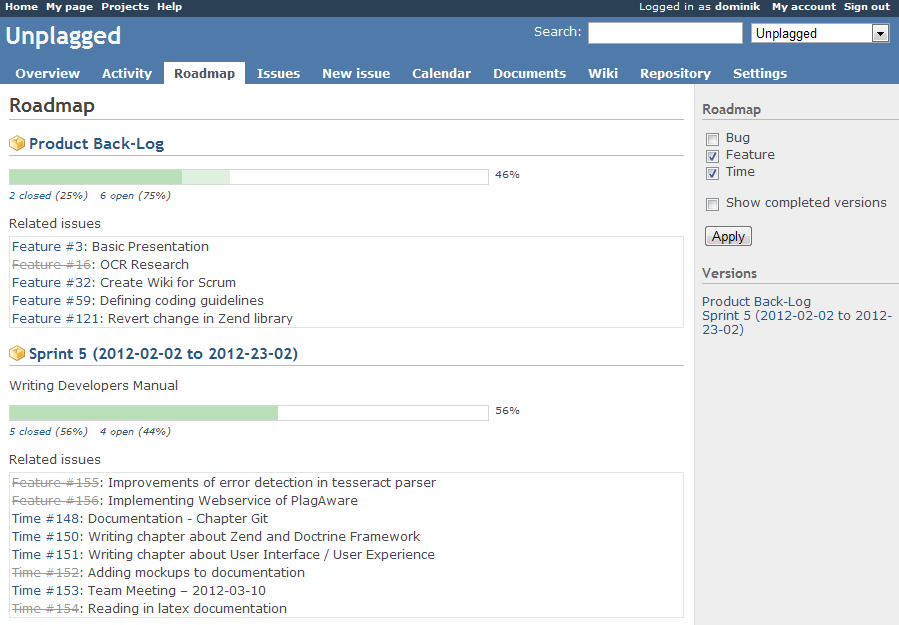
\includegraphics[width=\textwidth]{images/roadmap.png}
  \caption{Redmine Roadmap}
  \label{fig:roadmap}
\end{figure}

What we are doing there, is to map every \textit{Sprint} and the \textit{Product Backlog} to Redmine's notion of \enquote{Version} and
every identified \textit{User Story} to an \enquote{Issue}.

You can see in figure \ref{fig:roadmap} the view of the roadmap, with the current sprint 5 designated to create this very
document at the bottom and a not very well filled product backlog at the top. 

Normally 
every identified user story that is not part of the current sprint should be in the product backlog (and we got plenty), 
but as we were still working
in our small group at this point, the hassle of filling in all the tickets seemed unnecessary. This is something that
will be fixed in the near future, so that you are able to see where the development is going.

Currently we are working mostly with four week long sprints, to overcome the problem that we are not working fulltime
on the tickets, which is something that scrum normally assumes with its two week long sprints.

To have a nice statistical overview and more planning security for the \enquote{scrums}, it is required to log the time 
that was spent on an issue within redmine.

% Redmine description, Meetings, Debbie, Scrum Cards, Server, Website

\subsection{Product Owner --- \enquote{The Debbie Meetings}}

\begin{figure}[!h]
  \centering
    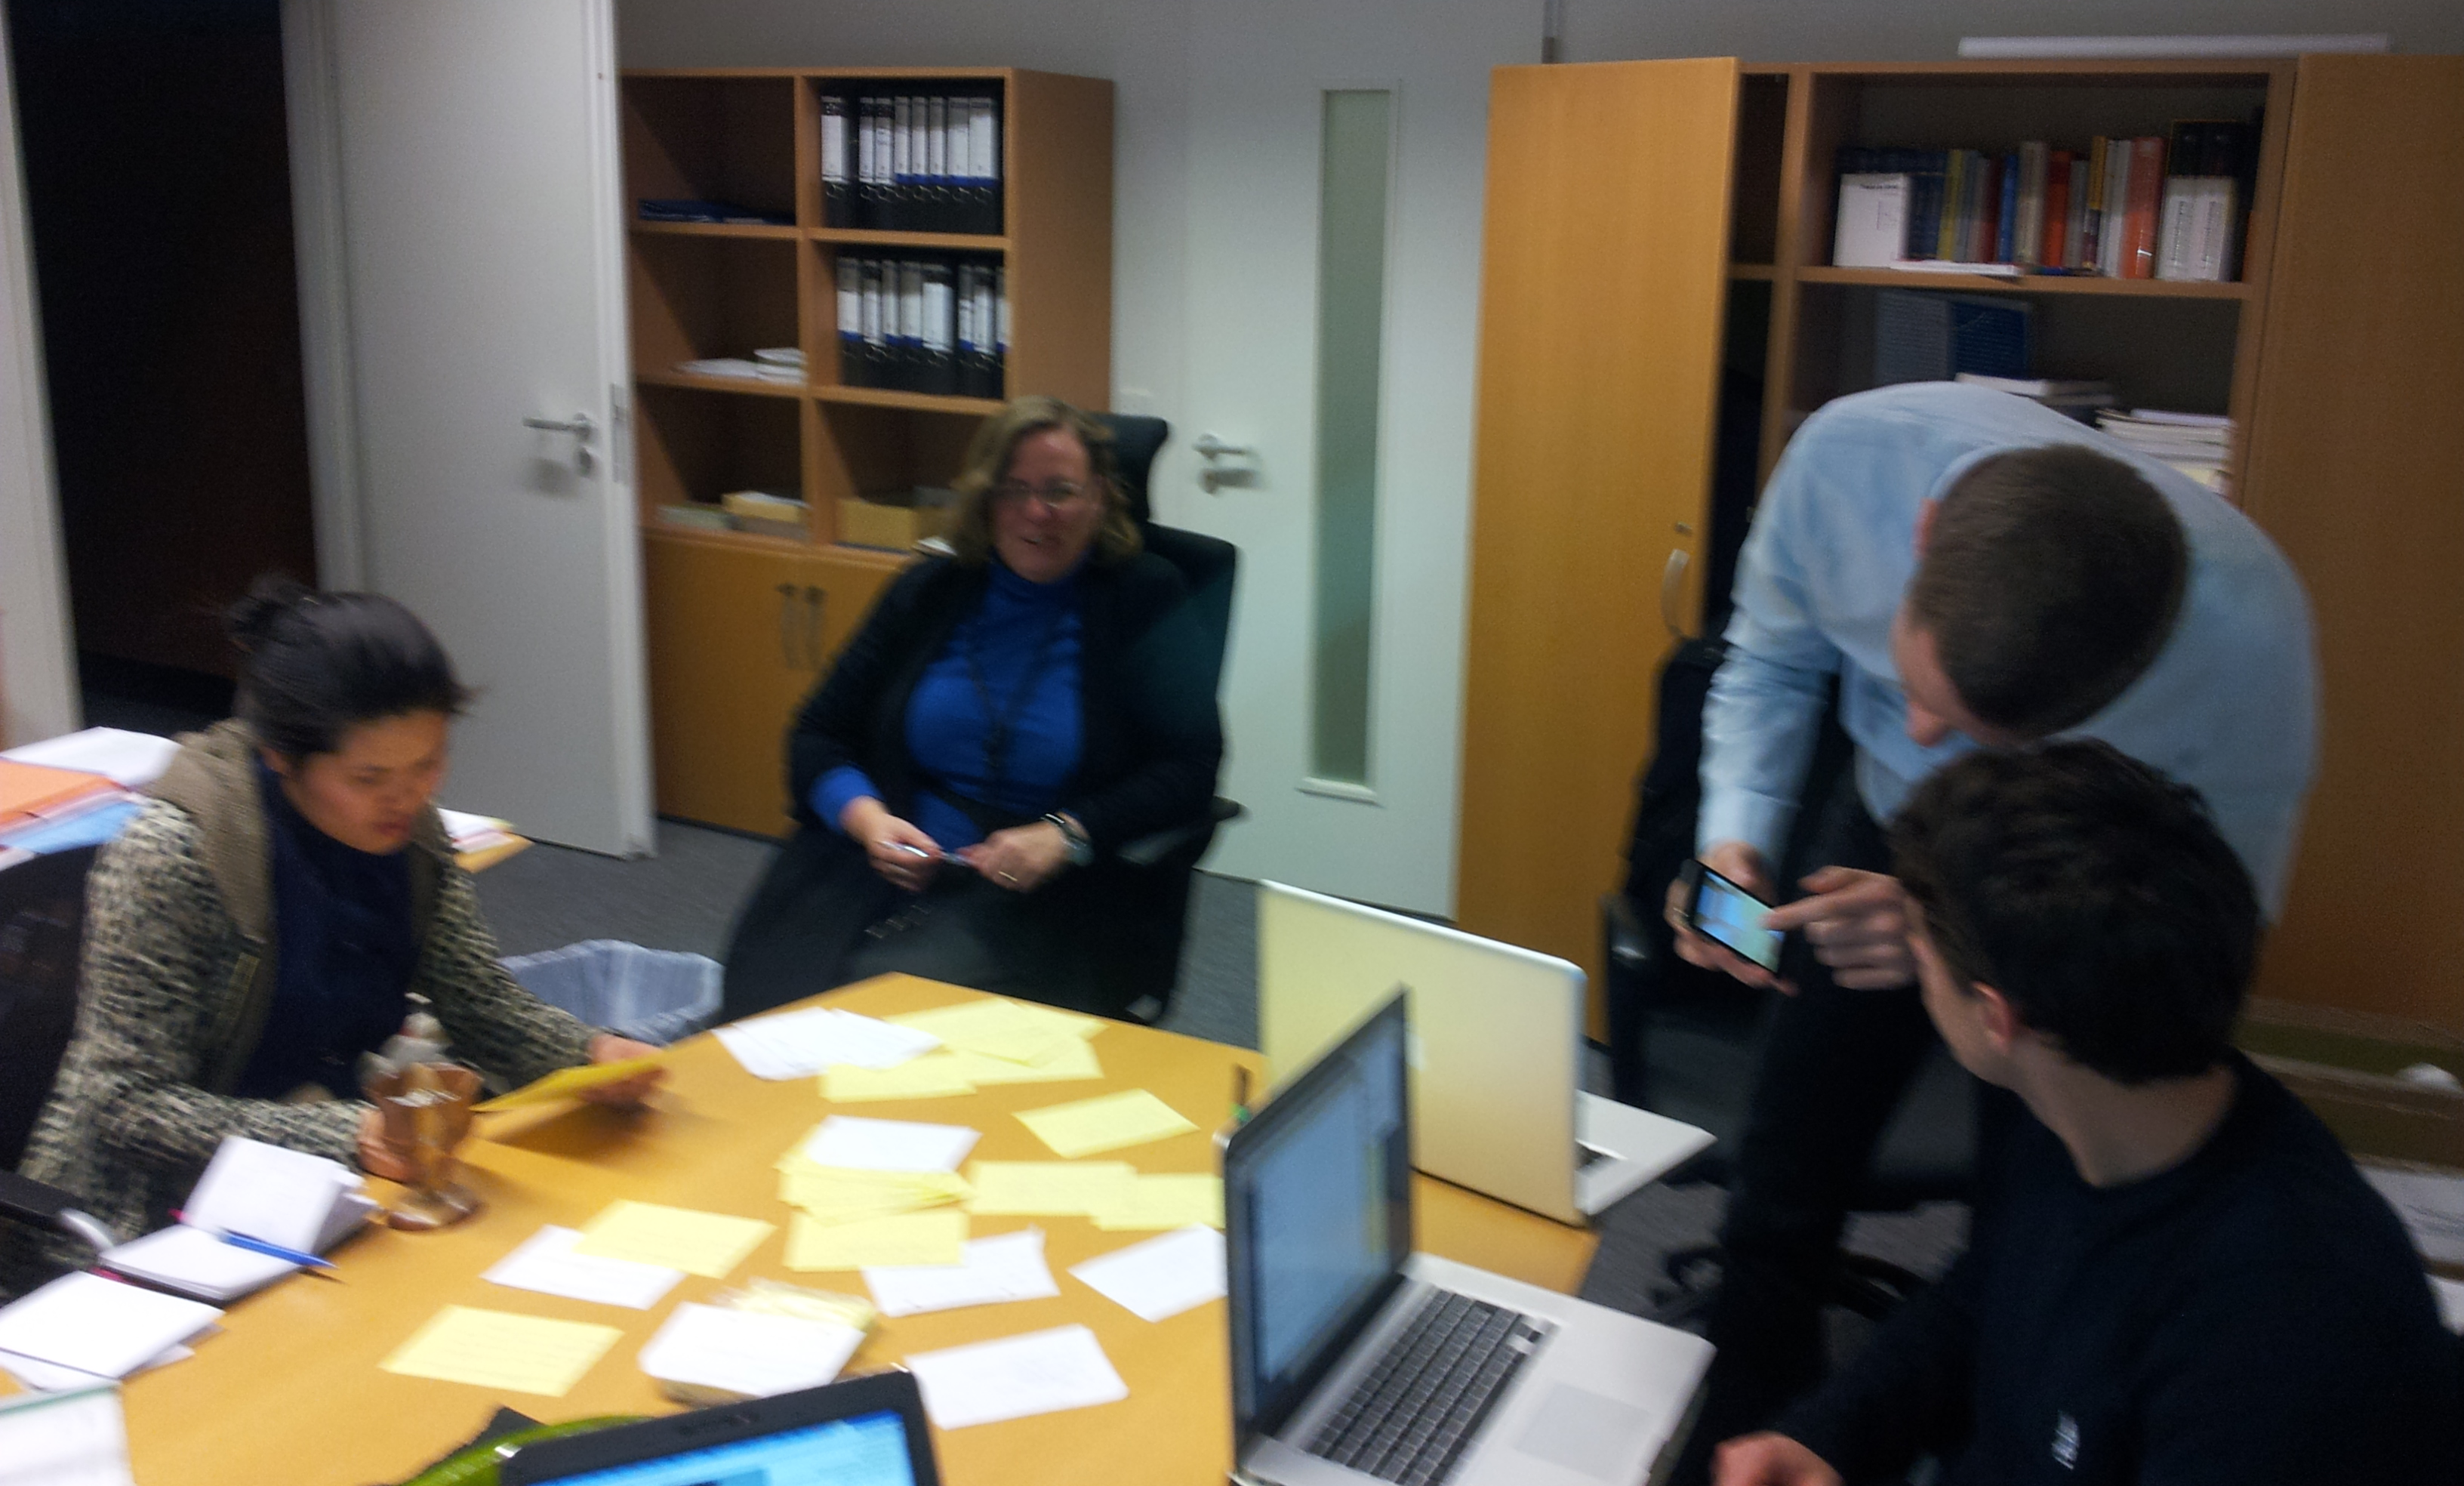
\includegraphics[width=0.8\textwidth]{images/2011-11-15-user-stories-6.jpg}
  \caption{Scrum Meeting}
  \label{fig:scrumming}
\end{figure}

To figure out the user stories we mostly rely on what we internally call \enquote{Debbie Meetings}.
Normally at the end of every sprint, the members of the team meet with Prof. Weber-Wulff, who we state to be our \textit{Product
Owner}. We simply sit down there and talk about what should be implemented in the next sprint and collect it on cards as
you can see in figure \ref{fig:userStories}.

We consider this to be just a temporary way of handling this, because we hope that when we eventually have a prototype 
that we consider to have enough \enquote{business value} to be shown to more people, the focus will shift away from 
Prof. Weber-Wulff to a more broader understanding of the product owner. 

\begin{figure}[!h]
  \centering
    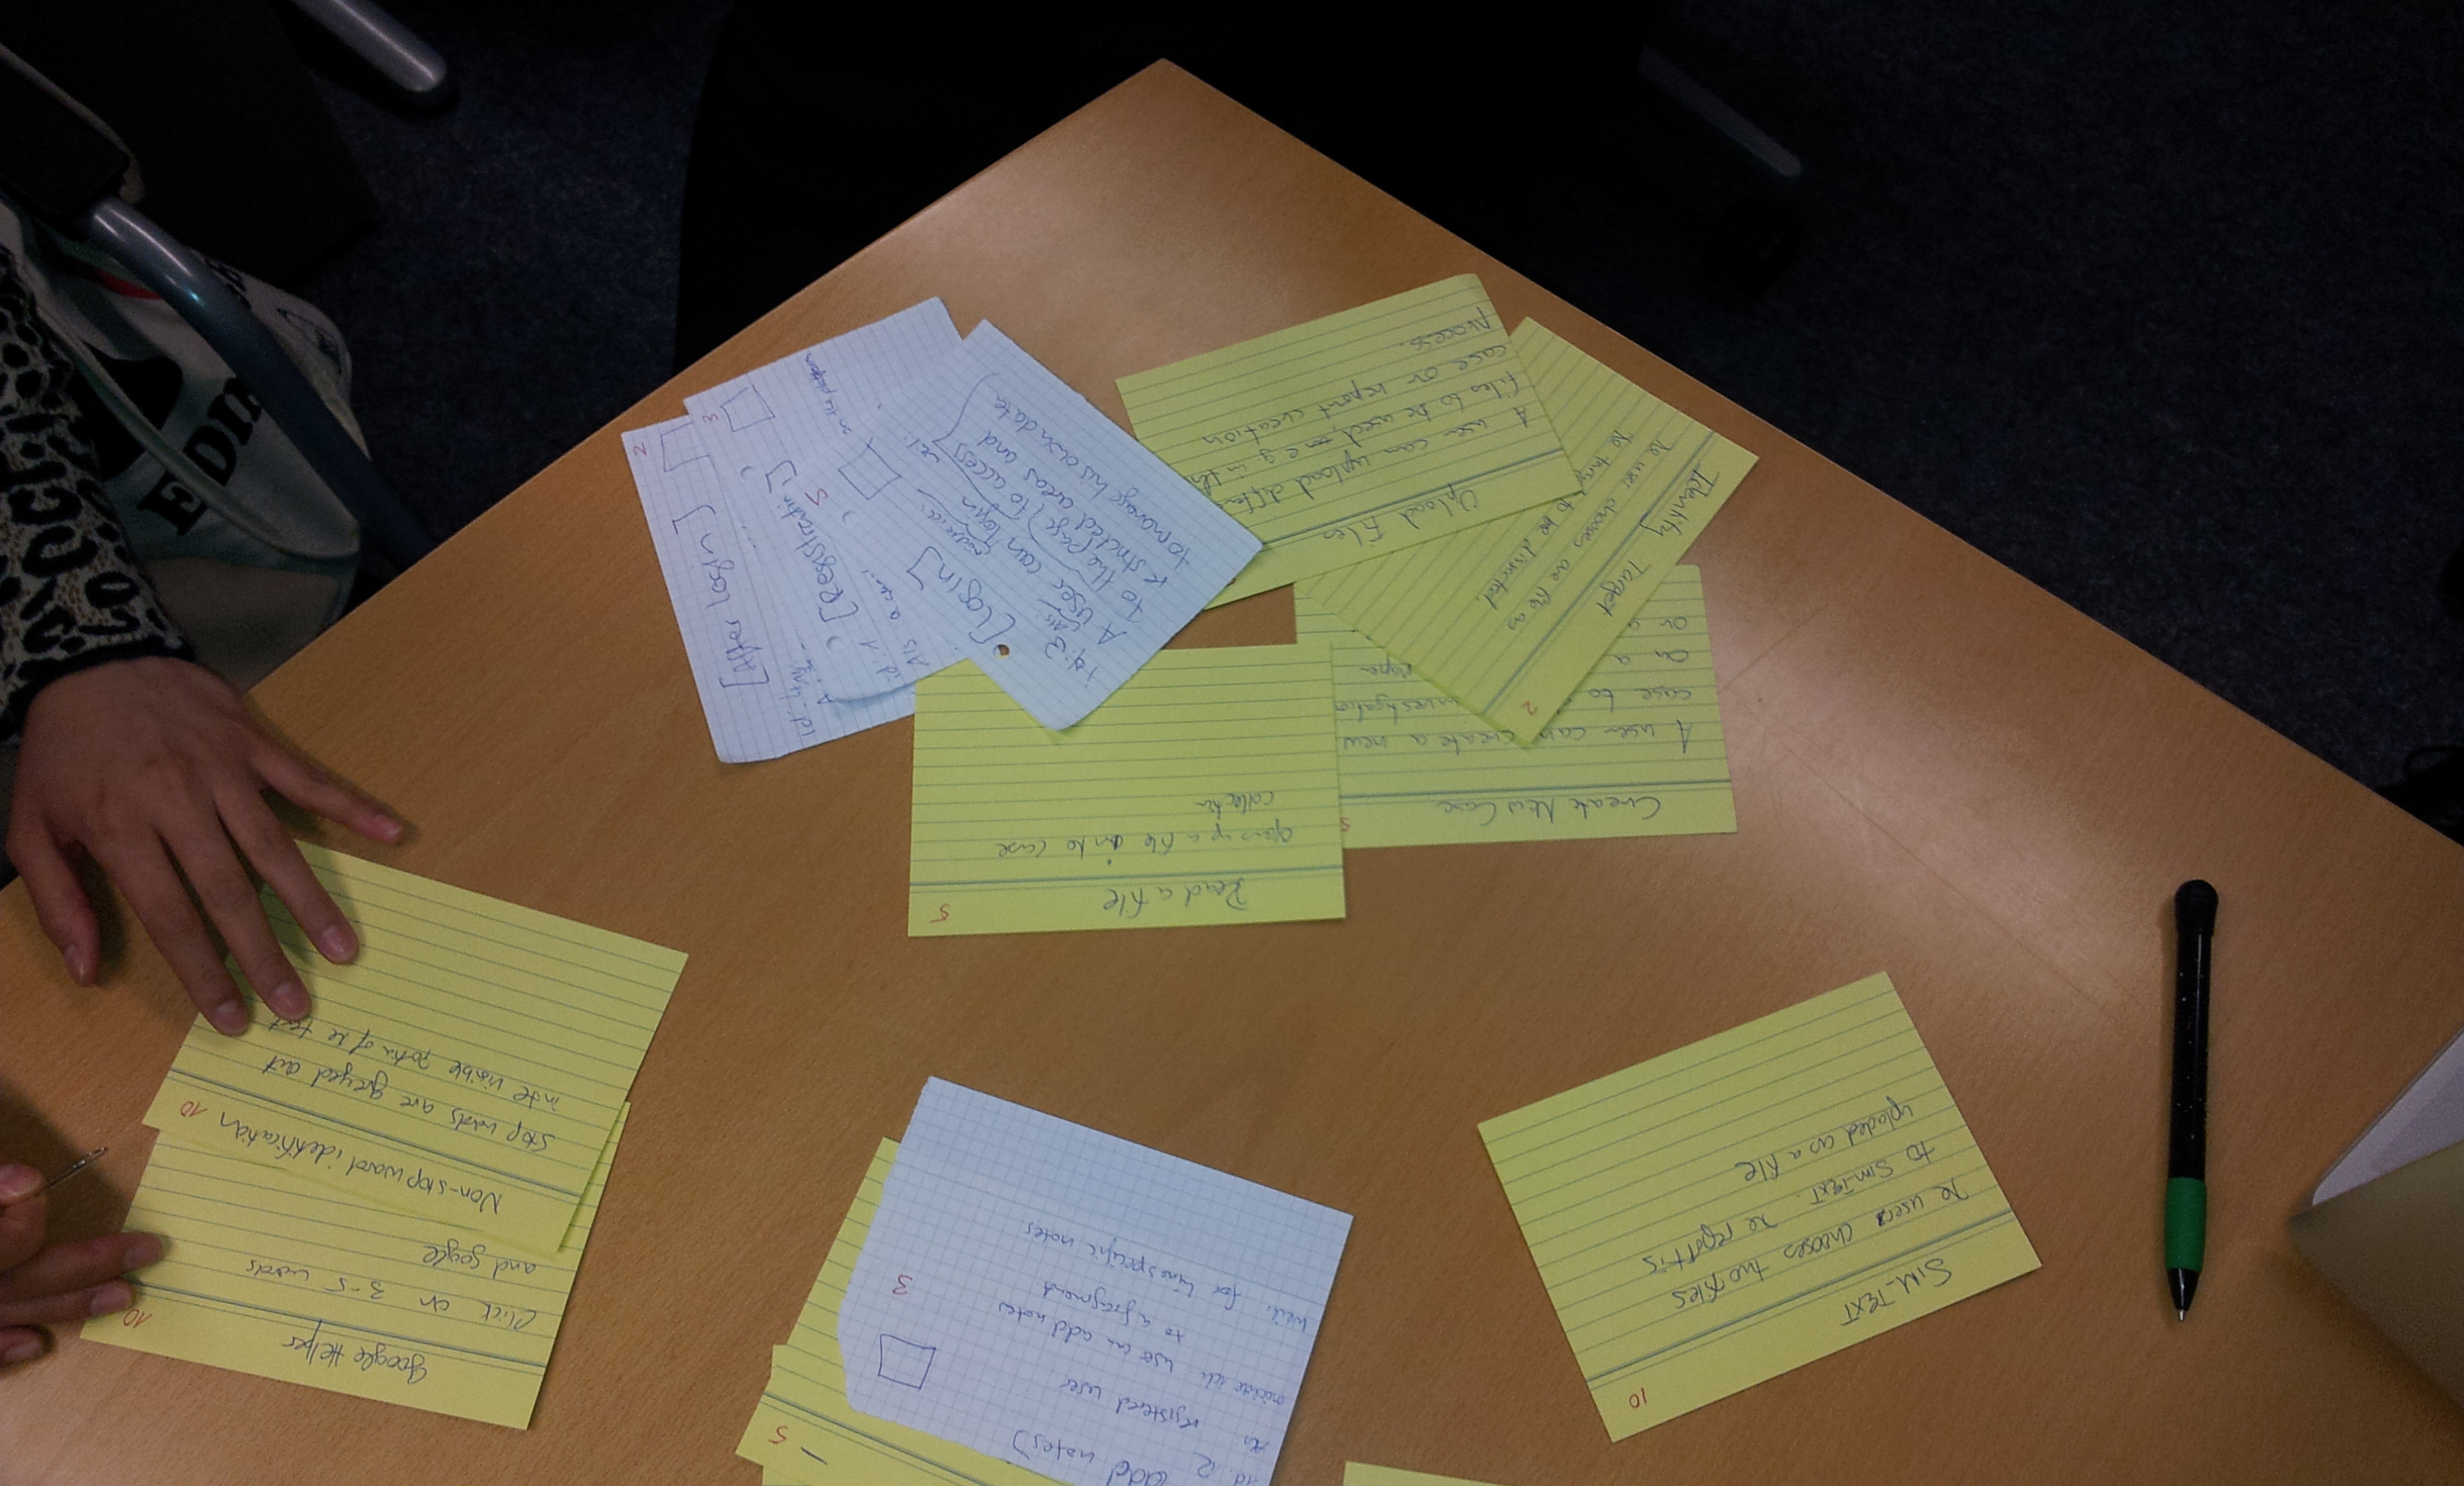
\includegraphics[width=0.8\textwidth]{images/2011-11-15-user-stories-4.jpg}
  \caption{User Stories}
  \label{fig:userStories}
\end{figure}

This means, that we want to open up our ticket system to directly collect new user stories and gather feedback for 
example from the VroniPlag group, which can be reached through their IRC channel \texttt{\#VroniPlag} on:

\begin{itemize}
\item \url{http://webchat.freenode.net/}
\end{itemize} 


\subsection{Team Meetings}

% I think it's better to use present tense, because the meetings will continue
The Unplagged version of the \textit{Daily Scrum} is currently a weekly meeting. Even though our meetings aren't daily, they 
are still respecting the other characteristics of a \textit{Daily Scrum}. Each team member says what was done in 
the last week and what is going to be done the next week. 

Those meetings are also the most problematic aspect of our version of Scrum, because the daily frequency of the 
meetings normally 
helps to let everybody know more about necessary changes in the logic of previously discussed ideas and makes the 
process
really agile. Sometimes this led to situations where team members developed unnecessary complicated, in a wrong direction
or not compatible with each other, which only got noticed a week later.

Our projectteam was doing the meetings every Monday for at least one hour. Most of the times we met at the same place, 
if due to appointment collisions we couldn't manage to meet in person, we met in Skype. So we never used to skip the 
weekly meeting.

% protocol is not really the same in english as Protokoll in german
For each meeting that we held someone was responsible for writing the minutes of the meeting. For each minutes a 
new wiki-page was created in \href{http://www.redmine.org/}{Redmine}. To put them into this tool
was really helpful for the teamwork, because everybody had access to it and could, 
if necessary, have a look at the decisions which were made in the past.

During the meetings at least these following points have been discussed:

\begin{itemize}
\item What was done last week 
\item What will be done for the next week
\item Time estimates of user stories
\item Organizational issues
\item External dependency issues
\item Problems encountered in the past
\item Further questions
\end{itemize}

All the minutes which were made during the first semester of the project are available in the appendix \ref{ch:Meetings} 
at page \pageref{ch:Meetings}.

\section{Target Group}

Our main target group is \textit{vroniplag}.
\minisec{}
But of course a goal of the application is also to support the detection of plagiarism for other groups as well. So the target group is composed of people who want to correct documents and be sure that this does not contain any plagiarism.

The following list is showing personas who could be interested in using this application:

\begin{itemize}
\item Professors 
\item Teachers
\item Academics
\item Instructors
\item Tutors
\item ...
\end{itemize}

These people are mostly not IT-specialists, so it is important to focus on it during the development of the application. This has an influence on the way they will use the application: it must be easy and naturally to use, the results must be easy to understand and reliable.

\section{Planned functionalities}
\subsection{System Requirements}

The following points describe some of the basic functionalities:

\begin{itemize}
\item Unplagged works in common modern browsers.
\item Unplagged works in common modern browsers.
\item The system can be used collaboratively, i. e. multiple users can work together on a case.
\item A user can provide input data for a case in different types of formats, e. g. pdf, jpeg, odt or doc.
\item A user can mark parts of the input data as fragments and store associated data, e. g. comments, plagiarism type or original source.
\item The users can create customizable reports for a case from the plagiarisms they found.
\item The system integrates OCR tools.
\item The reports can be generated in different types of output formats.
\item The system provides hooks to integrate plugins, for example to use different kinds of OCRs or to integrate intrinsic plagiarism detection.
\end{itemize}

And here it is broken down into the currently identified sections/modules of the system:

\subsection{Administration}

\begin{itemize}
\item Create, update and delete cases and users (User roles)
\end{itemize}

\subsection{Creating a new case}

Basic Information:
\begin{itemize}
\item Case Name
\item Probably an alias for the case
\item Visible to the public (yes/no) (if yes: show a hint "Project will be visible to anyone" and let user approve it)
\item Approvals needed (2 by default)
\end{itemize}

Suspect documents:
\begin{itemize}
\item Uploading documents belonging to the case
\end{itemize}

Collaborators:
\begin{itemize}
\item Name
\item Multiple groups with pre-defined right sets
\item Locked (whether the user is currently locked and can't do anything in the project or not)
\end{itemize}


\subsection{ Document Parser}

Take different kinds of documents or images and convert them into a common internal representation.

\subsection{ Editor Mode}

\subsubsection{ Detection modes}

Google Search - if no source is found yet
\begin{itemize}
\item Double click words in a suspect document
\item Do a Google-Search on it (left screen suspect document, right side of the screen: google search)
\item if something interesting is found on Google, open the source
\item Let user import the source into our system with bibtex information about the author and so on
\item Mark words in suspect document and imported source
\item Save as a new case
\end{itemize}

Sim
\begin{itemize}
\item Mark a browseable part in the suspect document and do a sim with a given source
\item Store result and highlight dif
\item Start creating fragments
\end{itemize}

Other sources
\begin{itemize}
\item Send suspicious document to a webservice and get back a report that can be used for further editing 
\end{itemize}

\subsection{Creating a candidate fragment}

Starting point:
\minisec{}
 by hand:
\begin{itemize}
\item Show suspect document on the left, possible source on the right
\item  Select parts on the left and right
\end{itemize}

detection mode
\begin{itemize}
\item automatically pre-marked text parts on each side, can be shifted
\end{itemize}

\begin{itemize}
\item Allow marking with different colors in one fragment
\item Multiple types can be added to each fragment  (Strukturplagiat, Bauernopfer,...)
\end{itemize}

Additional requirements:
Other sources
\begin{itemize}
\item Send suspicious document to a webservice and get back a report that can be used for further editing 
\item Merging multiple fragments
\item Marking a fragment over multiple pages
\item Mini Post-it on each line to add a specific note to a text part
\end{itemize}

Information:
\begin{itemize}
\item  A collection of page number, line number, word number of start and end  needs to be stored
\end{itemize}

\subsection{Approving a candidate fragment}
\begin{itemize}
\item  Show link to original source
\item show suspect part marked and show plagiarism type (Strukturplagiat, Bauernopfer,...) on the left
\item and source part on the right with marked text
\end{itemize}

\begin{itemize}
\item Add a comment and set a tick if approved or not
\item show stats how many people already approved or rejected the candidate fragment
\end{itemize}

\subsection{Report Generation}
\begin{itemize}
\item  drag and drop of fragment
\end{itemize}


\section{User roles}

As the Unplagged system will provide a permission based user system somewhere in the future, our goal is to make it 
possible, to create custom 
user roles from an administration area and make it possible for users to have multiple user roles in one case and also 
different roles for different cases.
The standard roles which will be provided by the system are:

\begin{description}
\item[Guest]
A user without a valid login can only see the parts of cases that are set to be public.
\item[Registered]
Registered users can get \enquote{promoted} to higher roles and contribute to publicly editable cases.
%Note: Do we want users to register themselves? Or do we have just an admin, that takes care of this? I'm currently also not sure if this will really need to be a role, or if Guest and Registerd are just two basic states.
\item[Collaborator]
Collaborators are registered users who were granted access to a specific case. Collaborators can access and edit these projects.
\item[Case-Manager]
Case-Managers can set up new cases and manage colloborators for their cases and project versions. They may have the permission to add or remmove project members.
%Note: What does manage project versions mean?
\item[Admin]
An admin owns all permissions, such as user administration or project administration. They also hvae the ability to to block/unblock an existing case.
\end{description}

\section{Current state of th basic functionalities}

The following points are showing the basic functionalities of the application.

\subsection{Register}

A person who wants to use the application needs to register first. The person then gets the ability to do it, as soon as opening the start-page and clicking the \enquote{Jetzt anmelden} link.

\begin{figure}[!ht]
  \centering
    
\includegraphics[width=0.50\textwidth]{images/basic_functionalities/reg1.png}
  \caption{Register link}
  \label{fig:register link}
\end{figure}

Below you see the register form which has to be filled.

\begin{figure}[!ht]
  \centering
    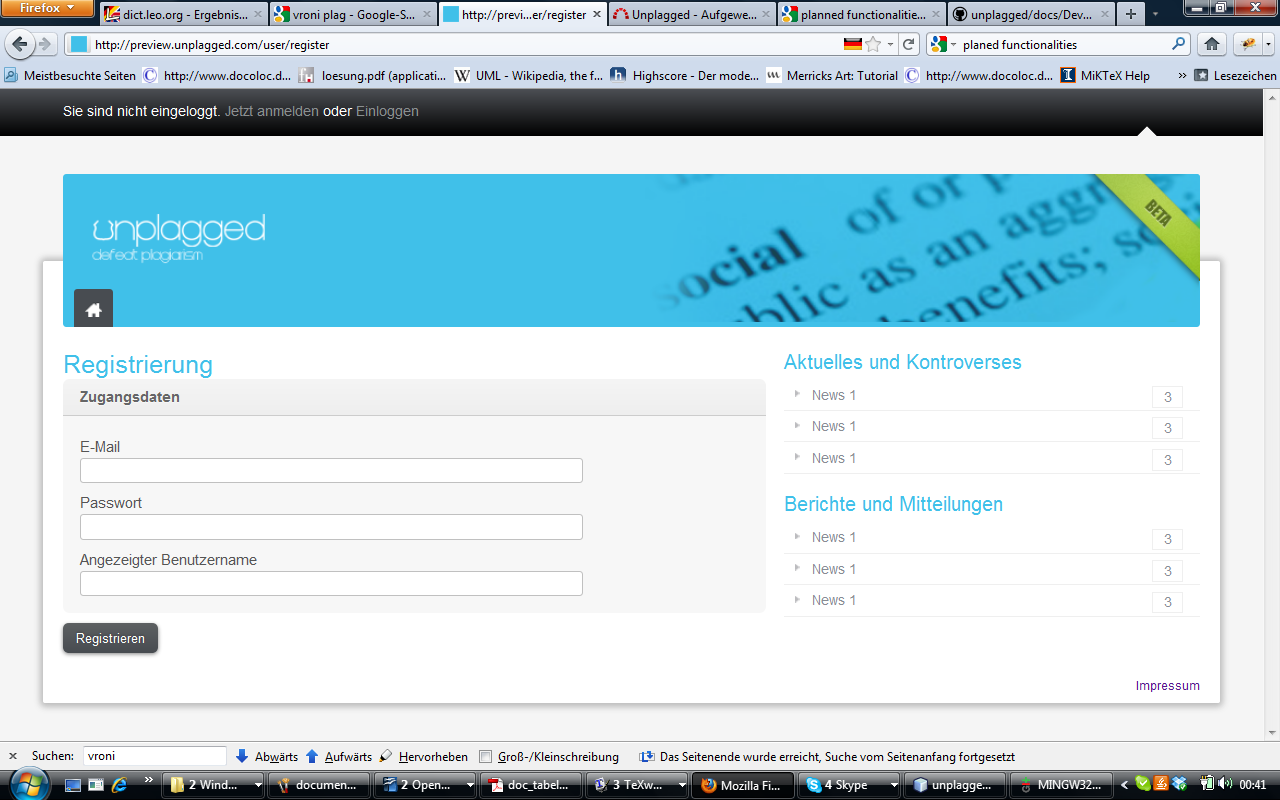
\includegraphics[width=0.97\textwidth]{images/basic_functionalities/register_form.png}
  \caption{Register form}
  \label{fig:register form}
\end{figure}

Every entry here will be saved in the database. Before the user can acutally login, a verification link sent to the email address, the user entered in the registration form, has to be opened. This prevents abuse and fake accounts at least a little.

\subsection{Login}

The login functionality is an easy to use form, which can be successfully used from every user which is already 
registered and verified. With a click on the "Einloggen" link, the login form will be visible.

\begin{figure}[!h]
  \centering
    
\includegraphics[width=0.30\textwidth]{images/basic_functionalities/oderEinloggen.png}
  \caption{"Einloggen" Link}
  \label{fig:einloggen}
\end{figure}

The received login data that are taken from the login form will be compared with the entries in the database, are the 
entries valid, the user has the right to use further functions in the application.

\begin{figure}[!h]
  \centering
    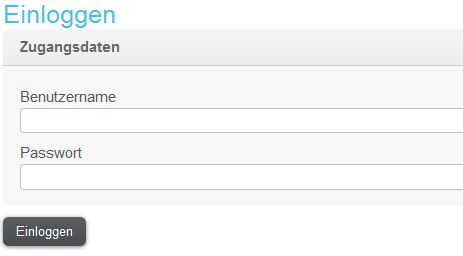
\includegraphics[width=0.97\textwidth]{images/basic_functionalities/login_form.png}
  \caption{Login form}
  \label{fig:einloggen}
\end{figure}

Below you see the view after the login.

\begin{figure}[!h]
  \centering
    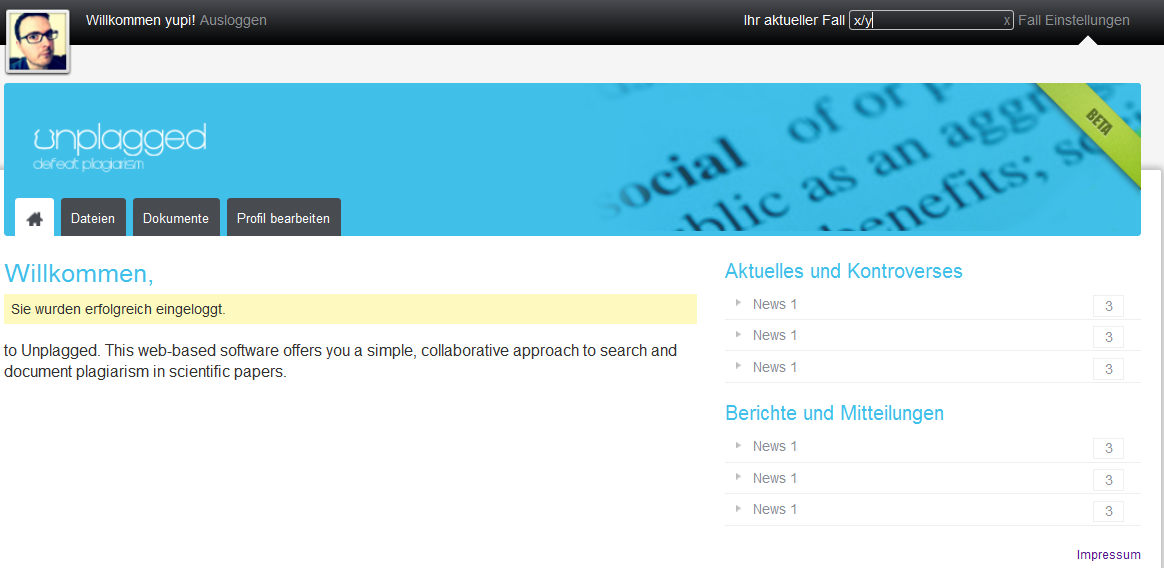
\includegraphics[width=0.97\textwidth]{images/basic_functionalities/after_login.png}
  \caption{After login view}
  \label{fig:after login view}
\end{figure}

\subsection{Create case}

To creat an own case the user only need to click on the \enquote{Fall Einstellungen} link.

\begin{figure}[!h]
  \centering
    
\includegraphics[width=0.30\textwidth]{images/basic_functionalities/case_options.png}
  \caption{Case options}
  \label{fig:case options}
\end{figure}


If the user has already some cases listed he can search for it in the searchfield. The field also shows the current case. This helps the user to orientate.
\begin{figure}[!h]
  \centering
    
\includegraphics[width=0.40\textwidth]{images/basic_functionalities/current_case_search_field.png}
  \caption{Current case and search field}
  \label{fig:current case and search field}
\end{figure}

\subsection{Files overview}

The tab \enquote{Dateien} is showing the list of files which were added from an user. Not only shows it an overview it 
also has several additionaly functions which can be processed on a file.

\begin{figure}[!h]
  \centering
    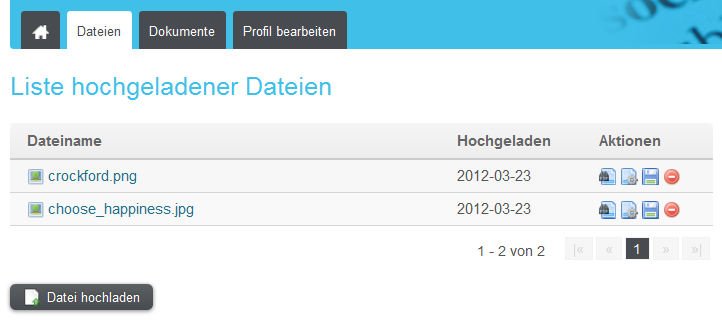
\includegraphics[width=0.97\textwidth]{images/basic_functionalities/dateien.png}
  \caption{Overview of files}
  \label{fig:overview of files}
\end{figure}

\subsubsection{Set target}

If the user wants to mark a specific file as his target file, he can do it just with a click on the following symbol.

\begin{figure}[!h]
  \centering
    
\includegraphics[width=0.05\textwidth]{images/page.png}
  \caption{File symbol}
  \label{fig: file symbol}
\end{figure}

\begin{figure}[!h]
  \centering
    
\includegraphics[width=0.97\textwidth]{images/basic_functionalities/set_target1.png}
  \caption{Not marked file}
  \label{fig:not marked file}
\end{figure}

Afterwards a binoculars icon will be shown.

\begin{figure}[!h]
  \centering
    
\includegraphics[width=0.97\textwidth]{images/basic_functionalities/set_target2.png}
  \caption{Marked target file}
  \label{fig:marked target file}
\end{figure}

\subsubsection{Parse}

The parse function parses the mentioned file and forwards the parsed file to the \enquote{Dokumente} section.
Witht a click of the following symbol, the parse function will be fired.

\begin{figure}[!h]
  \centering
    
\includegraphics[width=0.05\textwidth]{images/page_gear.png}
  \caption{Parse symbol}
  \label{fig:parse symbol}
\end{figure}

\subsubsection{Download}

With the disk-symbol the user can download the listed file.

\begin{figure}[!h]
  \centering
    
\includegraphics{images/disk.png}
  \caption{Download symbol}
  \label{fig: download symbol}
\end{figure}

\subsubsection{Delete}

To delete a file the user only needs to click on the following symbol.

\begin{figure}[!h]
  \centering
    
\includegraphics[width=0.05\textwidth]{images/basic_functionalities/delete.png}
  \caption{Delete symbol}
  \label{fig: ddelete symbol}
\end{figure}

After the function was fired the path to the file in the database and the file in the related folder will be deleted.

\subsubsection{File upload}

The file uploader is a important function, it gives the user the opportunity to upload data which he wants to work on. The user also has the opportunity to give the file a desired name.


\begin{figure}[!ht]
  \centering
    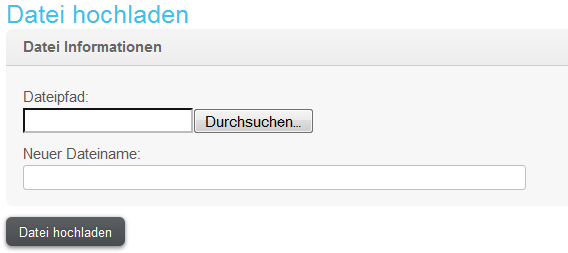
\includegraphics[width=0.97\textwidth]{images/basic_functionalities/datei_hochladen.png}
  \caption{File uploader}
  \label{fig:file uploader}
\end{figure}

\subsection{Parsed files overview}\label{sec:parse-file}

So after a file was parsed with the parse function from the \enquote{Dateien} section, it will be listed in the 
\enquote{Dokumente} tab.

\begin{figure}[!ht]
  \centering
    
\includegraphics[width=0.97\textwidth]{images/basic_functionalities/dokumente.png}
  \caption{List of parsed documents}
  \label{fig: List of parsed documents}
\end{figure}

The following functions are provided there for the user.

\subsubsection{Integration of detection plagiarism software}

The \enquote{plag-detection} functionality gives user the possibility to check a parsed file of plagiarism automatically. 
It uses the application interface from the company \enquote{PlagAware}. This is possible during our coorporation with 
\enquote{PlagAware}.
With the following symbol the \enquote{plag-detection} function can be used on the file.The detailed result report is 
not to see on the application. But the user has the possibility to see it on the \enquote{PlagAware} page.The user can get 
several informations on the application, like the success of the scanning and the procentaged part of the plagiarism.

\begin{figure}[!ht]
  \centering
    
\includegraphics[width=0.05\textwidth]{images/eye.png}
  \caption{Detect plagiarism symbol}
  \label{fig:detect plagiarism symbol}
\end{figure}

\subsubsection{Delete}

To delete a parsed file the user only needs to click on the following symbol.

\begin{figure}[!ht]
  \centering
    
\includegraphics[width=0.05\textwidth]{images/delete.png}
  \caption{Delete symbol}
  \label{fig:delete symbol}
\end{figure}

After the function was fired the path to the file in the database and the file in the related folder will be deleted.
\minisec{}

As soon as the user clicks on a listed document, the parsed pages of the documents will be shown. In this area the user has several functions which he can use to a page. This functions are followed listed.

\subsubsection{De-hyphen}
If a word is at the end of a line to long to fit in the line, one half of the word gets a hyphen. This function marks those sentence. So for the user such broken words are easy to detect.
\begin{figure}[!ht]
  \centering
    
\includegraphics[width=0.05\textwidth]{images/basic_functionalities/text_padding_right.png}
  \caption{De-hyphen function symbol}
  \label{fig:De-hyphen function symbol}
\end{figure}

\subsubsection{Stopwords}
Stopwords are disturbing or not so interesting parts in texts for plagiarism. Thats why the user can gray them out with this functionality.
\begin{figure}[!ht]
  \centering
    
\includegraphics[width=0.05\textwidth]{images/basic_functionalities/zoom.png}
  \caption{Stopword function symbol}
  \label{fig:stopword function symbol}
\end{figure}


\subsubsection{Plagiarism detection reports}
With this function the user has the possibility to see the reports, which were created by a plagiarism detection software.
\begin{figure}[!ht]
  \centering
    
\includegraphics[width=0.05\textwidth]{images/basic_functionalities/report_magnify.png}
  \caption{Plagiarism detection reports symbol}
  \label{fig:plagiarism detection reports symbol}
\end{figure}


\subsubsection{Edit}
The user hast the possibility to edit the text of the page.
\begin{figure}[!ht]
  \centering
    
\includegraphics[width=0.05\textwidth]{images/basic_functionalities/pencil.png}
  \caption{Edit symbol}
  \label{fig:edit symbol}
\end{figure}

\subsubsection{Delete}
The user can delete the desired page.
\begin{figure}[!ht]
  \centering
    
\includegraphics[width=0.05\textwidth]{images/basic_functionalities/delete.png}
  \caption{Delete symbol}
  \label{fig:delete symbol}
\end{figure}

\subsubsection{Simtext}

The simtext function is meant to compare two files with each other. So equal parts in texts can be detected.

\begin{figure}[!ht]
  \centering
    
\includegraphics[width=0.97\textwidth]{images/basic_functionalities/simtext_running.png}
  \caption{Simtext running example}
  \label{fig: Simtext running example}
\end{figure}

The simtext function also creates a report, where further detailed information can be seen.

\begin{figure}[!ht]
  \centering
    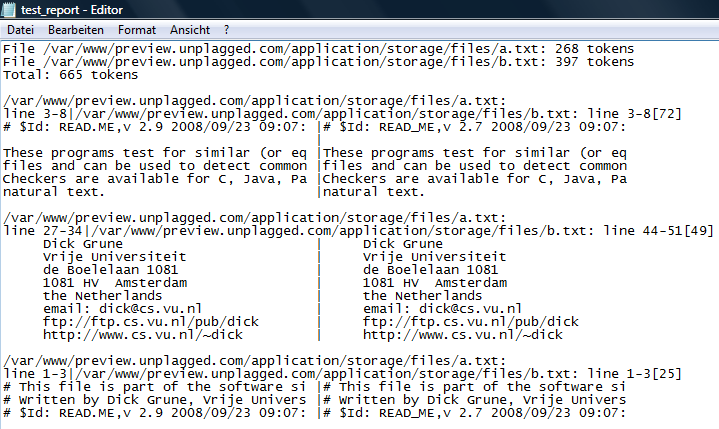
\includegraphics[width=0.97\textwidth]{images/basic_functionalities/simtext_report.png}
  \caption{Example of a Simtex report}
  \label{fig:example simtex report}
\end{figure}

In the report the equal parts on the compared files are shown.

\subsection{Edit profile}

The \enquote{Profil bearbeiten} form is a form which gives the user the opportunity to change profile informations that 
he gave before. All edit and saved entries will be saved in the database.

\begin{figure}[!ht]
  \centering
    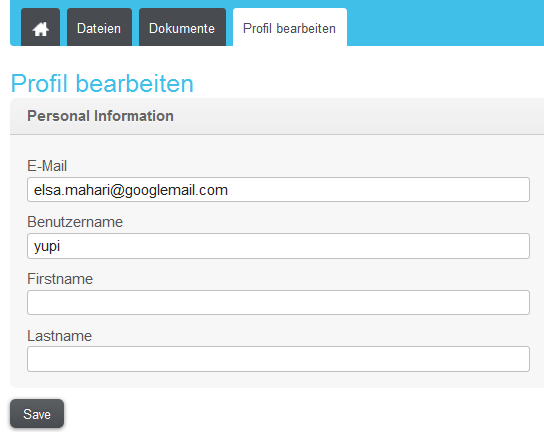
\includegraphics[width=0.97\textwidth]{images/basic_functionalities/edit_profile.png}
  \caption{Profile edit form}
  \label{fig: profile edit form}
\end{figure}

\subsection{Googlesearch}

The \enquote{Googlesearch} function is content from the contextmenu of the application. The contextmenu only shows if 
the user marked text on the application. So the user can direclty search for text in google from the application. After 
the searchwords the user have to click on \enquote{Goolge-Suchwörter löschen}.

\begin{figure}[!ht]
  \centering
    
\includegraphics[width=0.97\textwidth]{images/basic_functionalities/contextmenu_googlesearch.png}
  \caption{Googlesearch contextmenu}
  \label{fig:contextmenu}
\end{figure}

\subsection{Document Parser}

The document parser is more of a background functionality that enables a user to input data into the system. 
Essentially it is only an interface, that can be used to implement converters for different types of data, e. g images 
of scanned texts, PDFs, Word documents 
or similar, into an internal representation of a 
document.  

Currently this is used when a user uploads an image of scanned text and tries to parse it as described in section 
\nameref{sec:parse-file}.



\chapter{Developing Unplagged}\label{chap:developingUnplagged}

\section{Installation}
\subsection{Tesseract}
\subsection{Simtext}
\subsection{Imagemagick}

\section{Development Environment}

\subsection{Git}
\subsection{Netbeans}
\subsection{Staging and Preview System}

\section{Architectural Goals}

\subsection{Progressive Enhancement}

\subsection{Test Driven Development}

\subsection{Responsive Design}

\begin{appendix}

\chapter{Sprints}

\chapter{Minutes}

\chapter{Logged Time As Of March 11, 2012}
% should be updated later on, now simply to make sure it works
% generate various reports in redmine and export as csv
% don't forget to escape special characters like _ or # in the input .csv with \_ or \#


\DTLloaddb{overview}{data/timelog-overview.csv}
\begin{table}[htbp]
  \caption{Overview By Member and Month}
  \centering
  \DTLdisplaydb{overview}
\end{table}

\begin{landscape}

\DTLsetseparator{,}

\DTLloaddb{issueMember}{data/timelog-issue-member.csv}
  \centering
 \DTLdisplaylongdb[caption="Overview By Member and Issue"]{issueMember}

\DTLloaddb{sprints}{data/timelog-sprints.csv}
\begin{table}[htbp]
  \caption{Overview By Sprints}
  \centering
  \DTLdisplaydb{sprints}
\end{table}

\end{landscape}

\chapter{Mockups}

\section{Hand-Drawn}

\begin{figure}[!h]
  \centering
    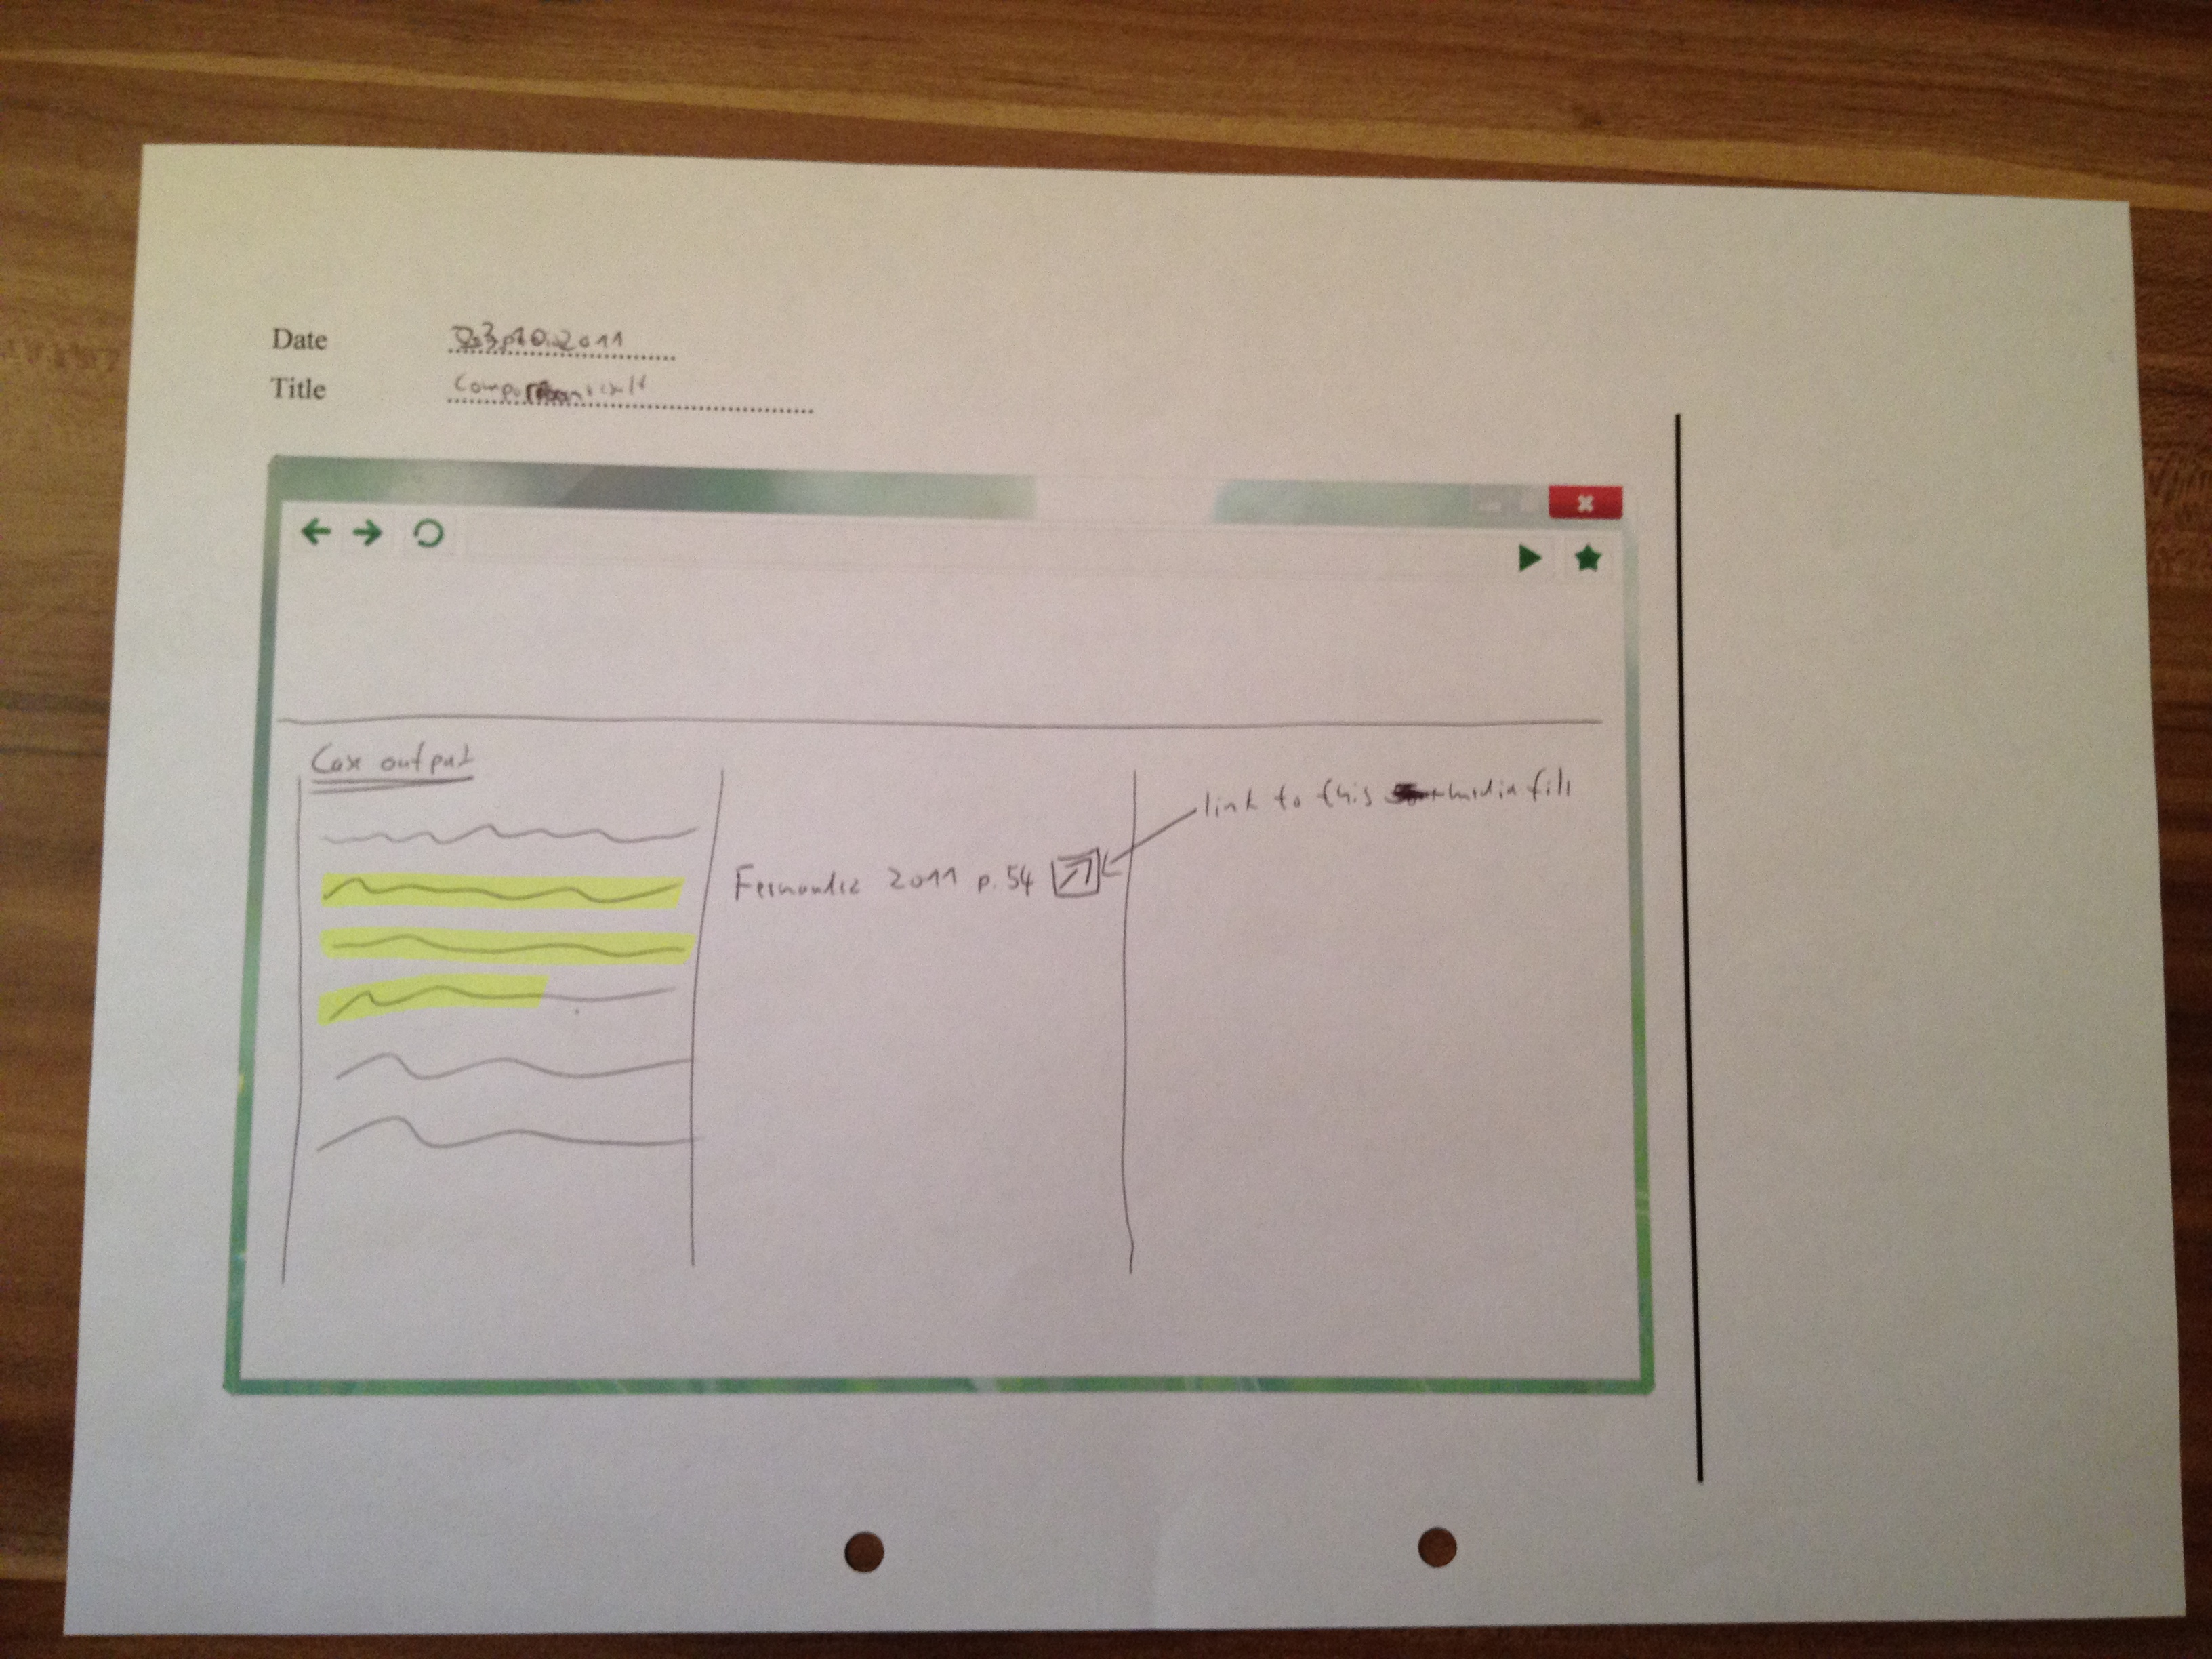
\includegraphics[width=\textwidth]{mockups/m_compare_result.jpg}
  \caption{Mockup – Compare results – digitalized }
  \label{fig:mCompareResultsMockup}
\end{figure}

\begin{figure}[!h]
  \centering
    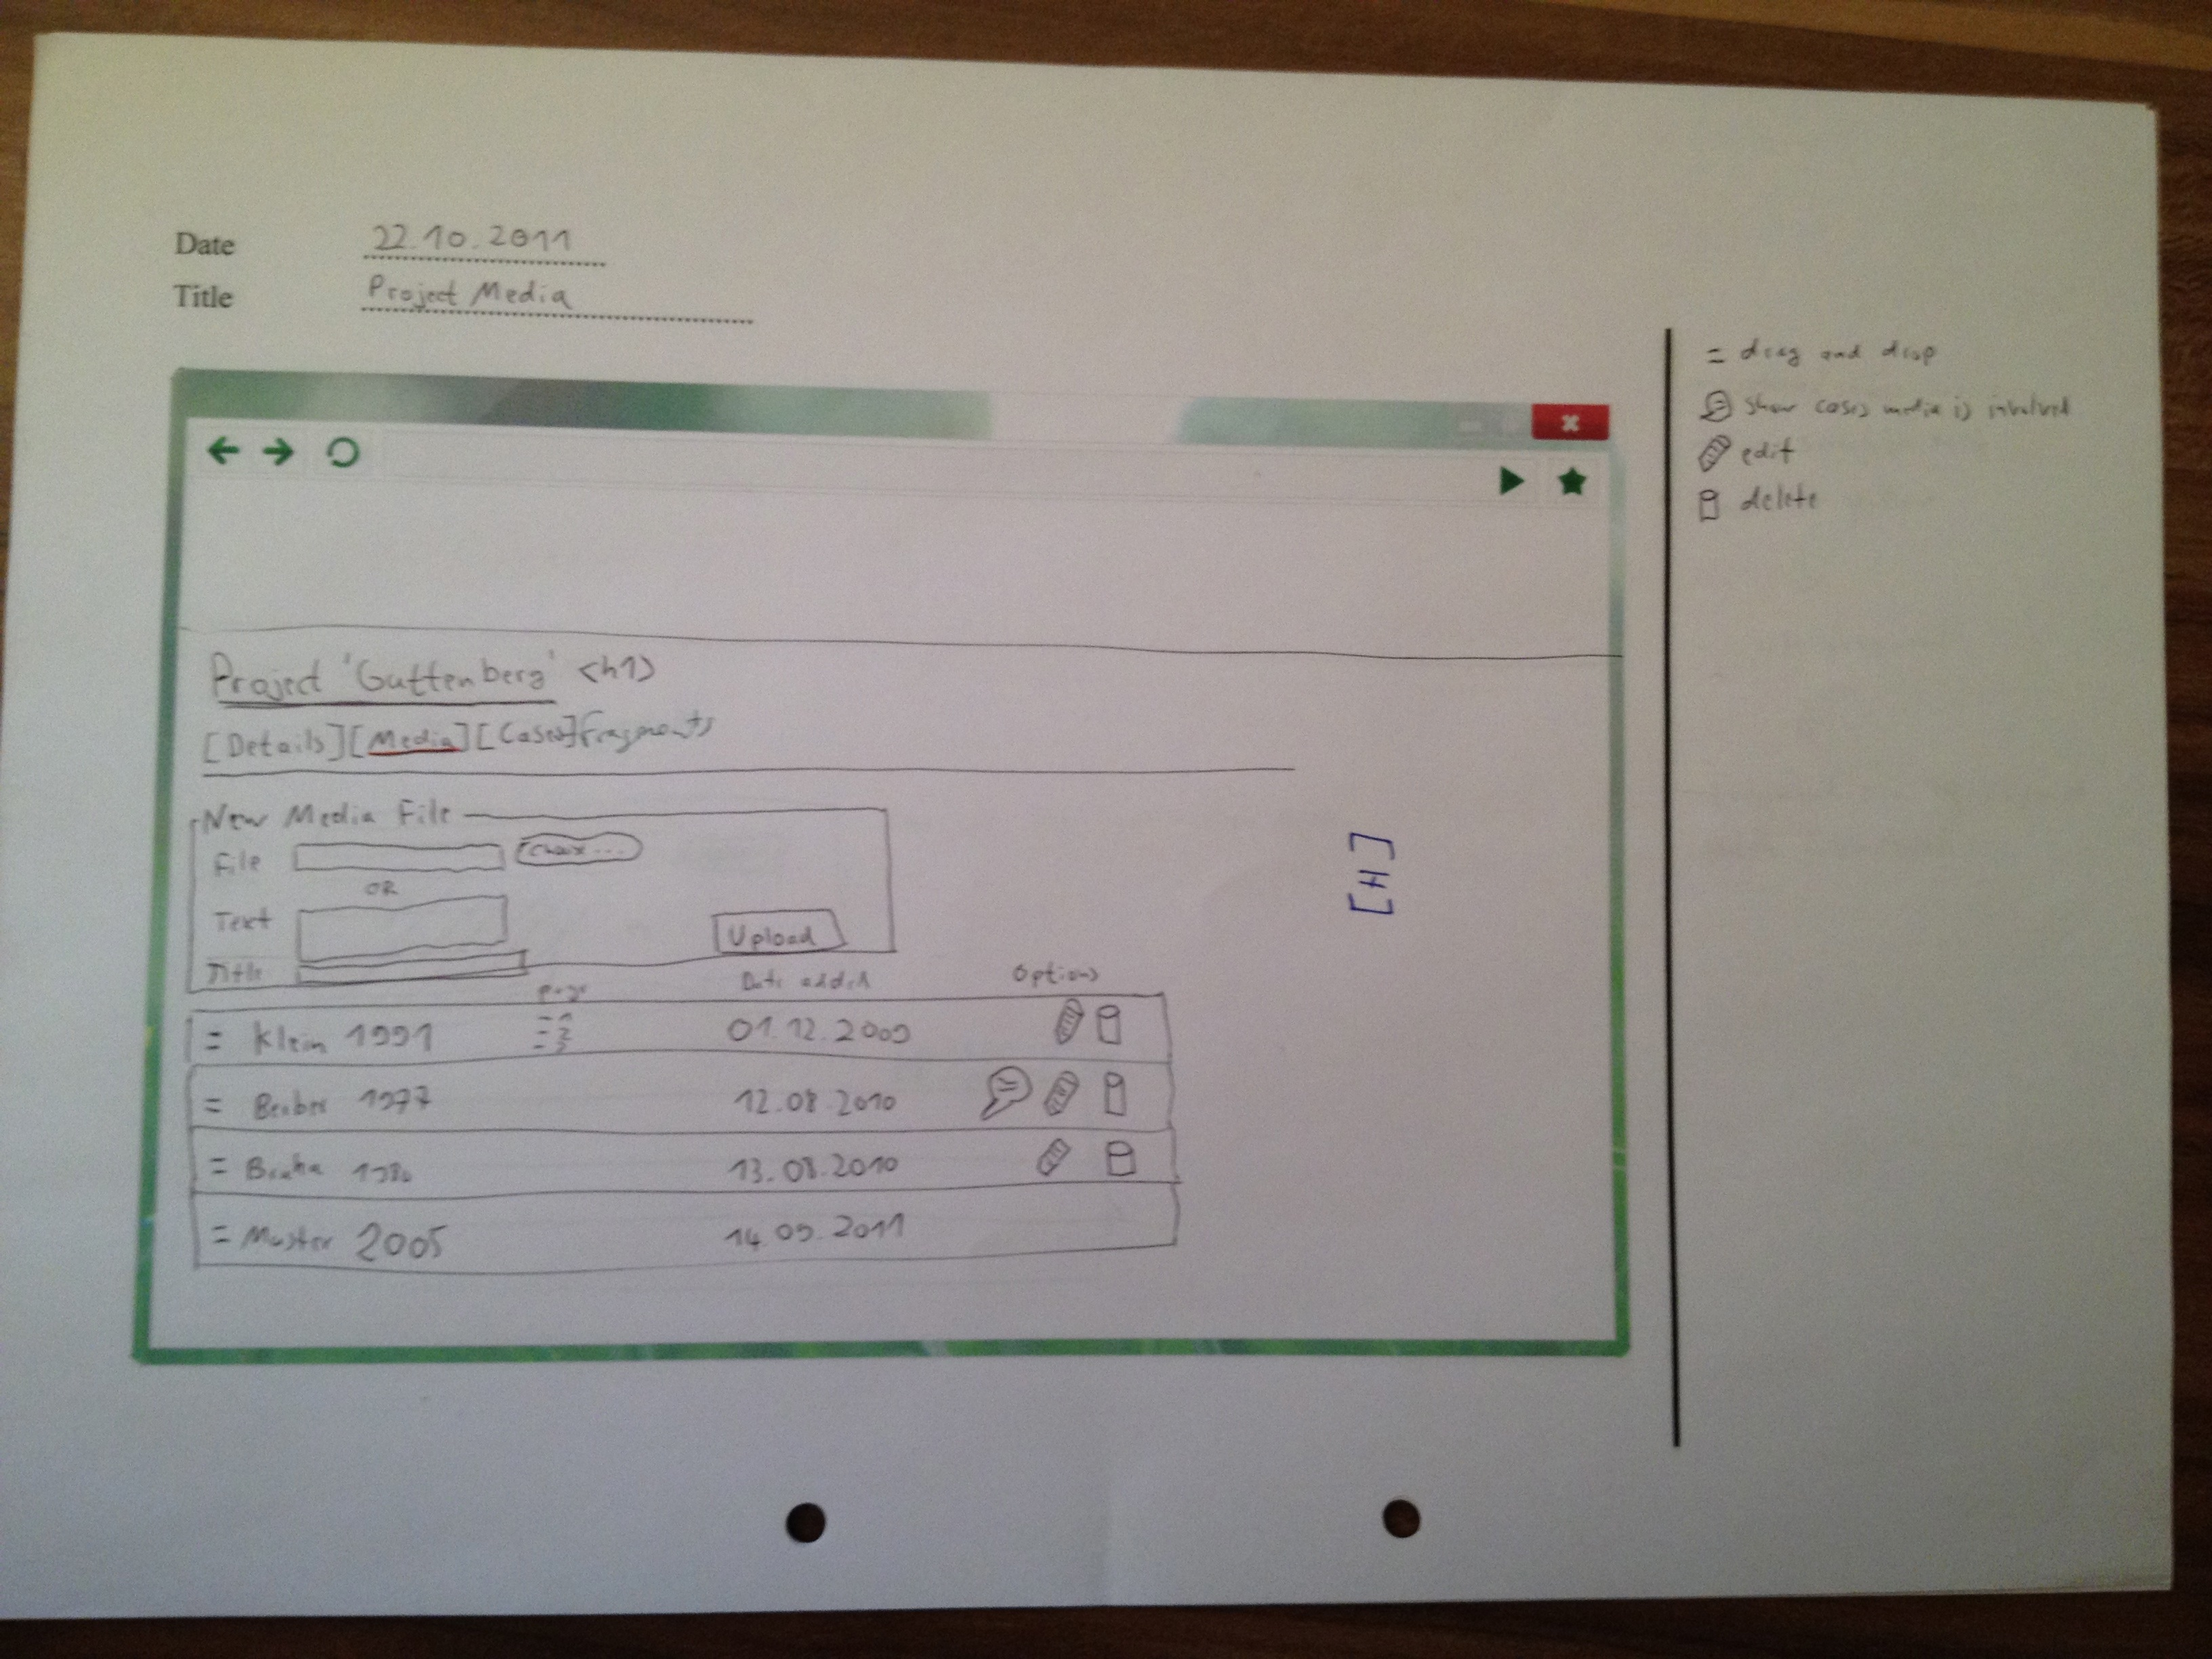
\includegraphics[width=\textwidth]{mockups/m_media_list.jpg}
  \caption{Mockup – Media list – digitalized }
  \label{fig:mMediaListMockup}
\end{figure}

\begin{figure}[!h]
  \centering
    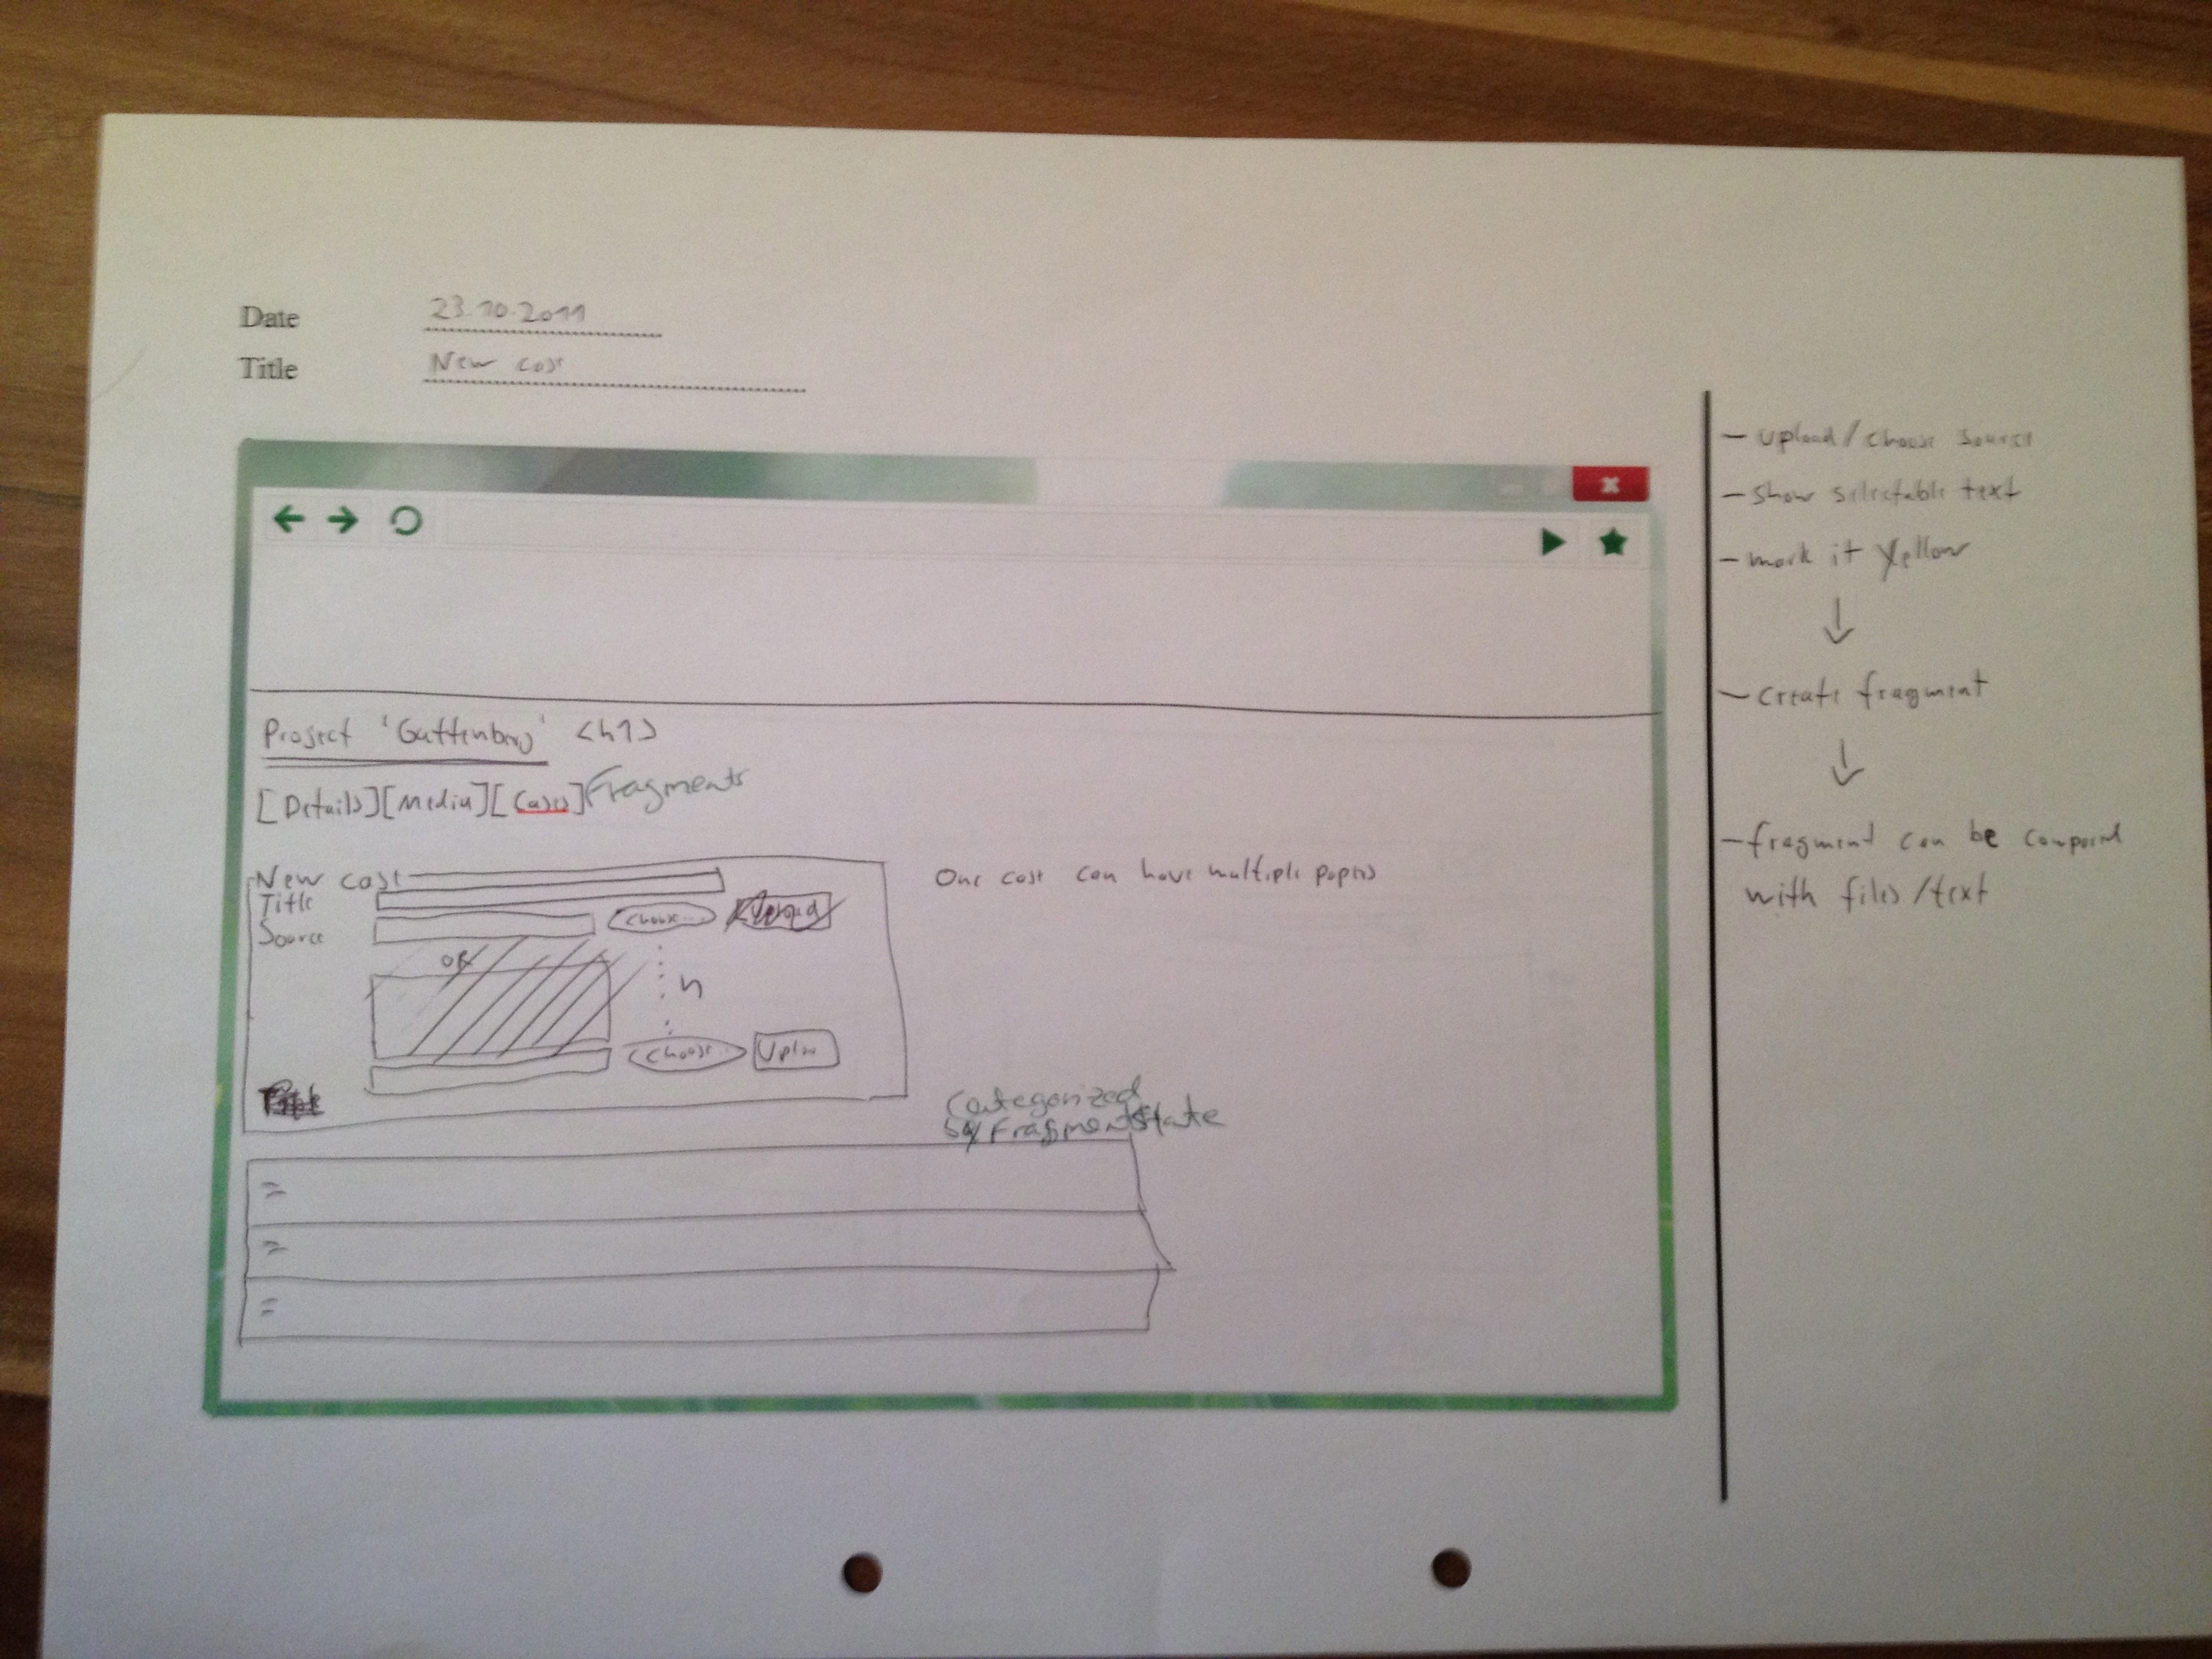
\includegraphics[width=\textwidth]{mockups/m_new_case.jpg}
  \caption{Mockup – New case – digitalized }
  \label{fig:1newCaseMockup}
\end{figure}

\begin{figure}[!h]
  \centering
    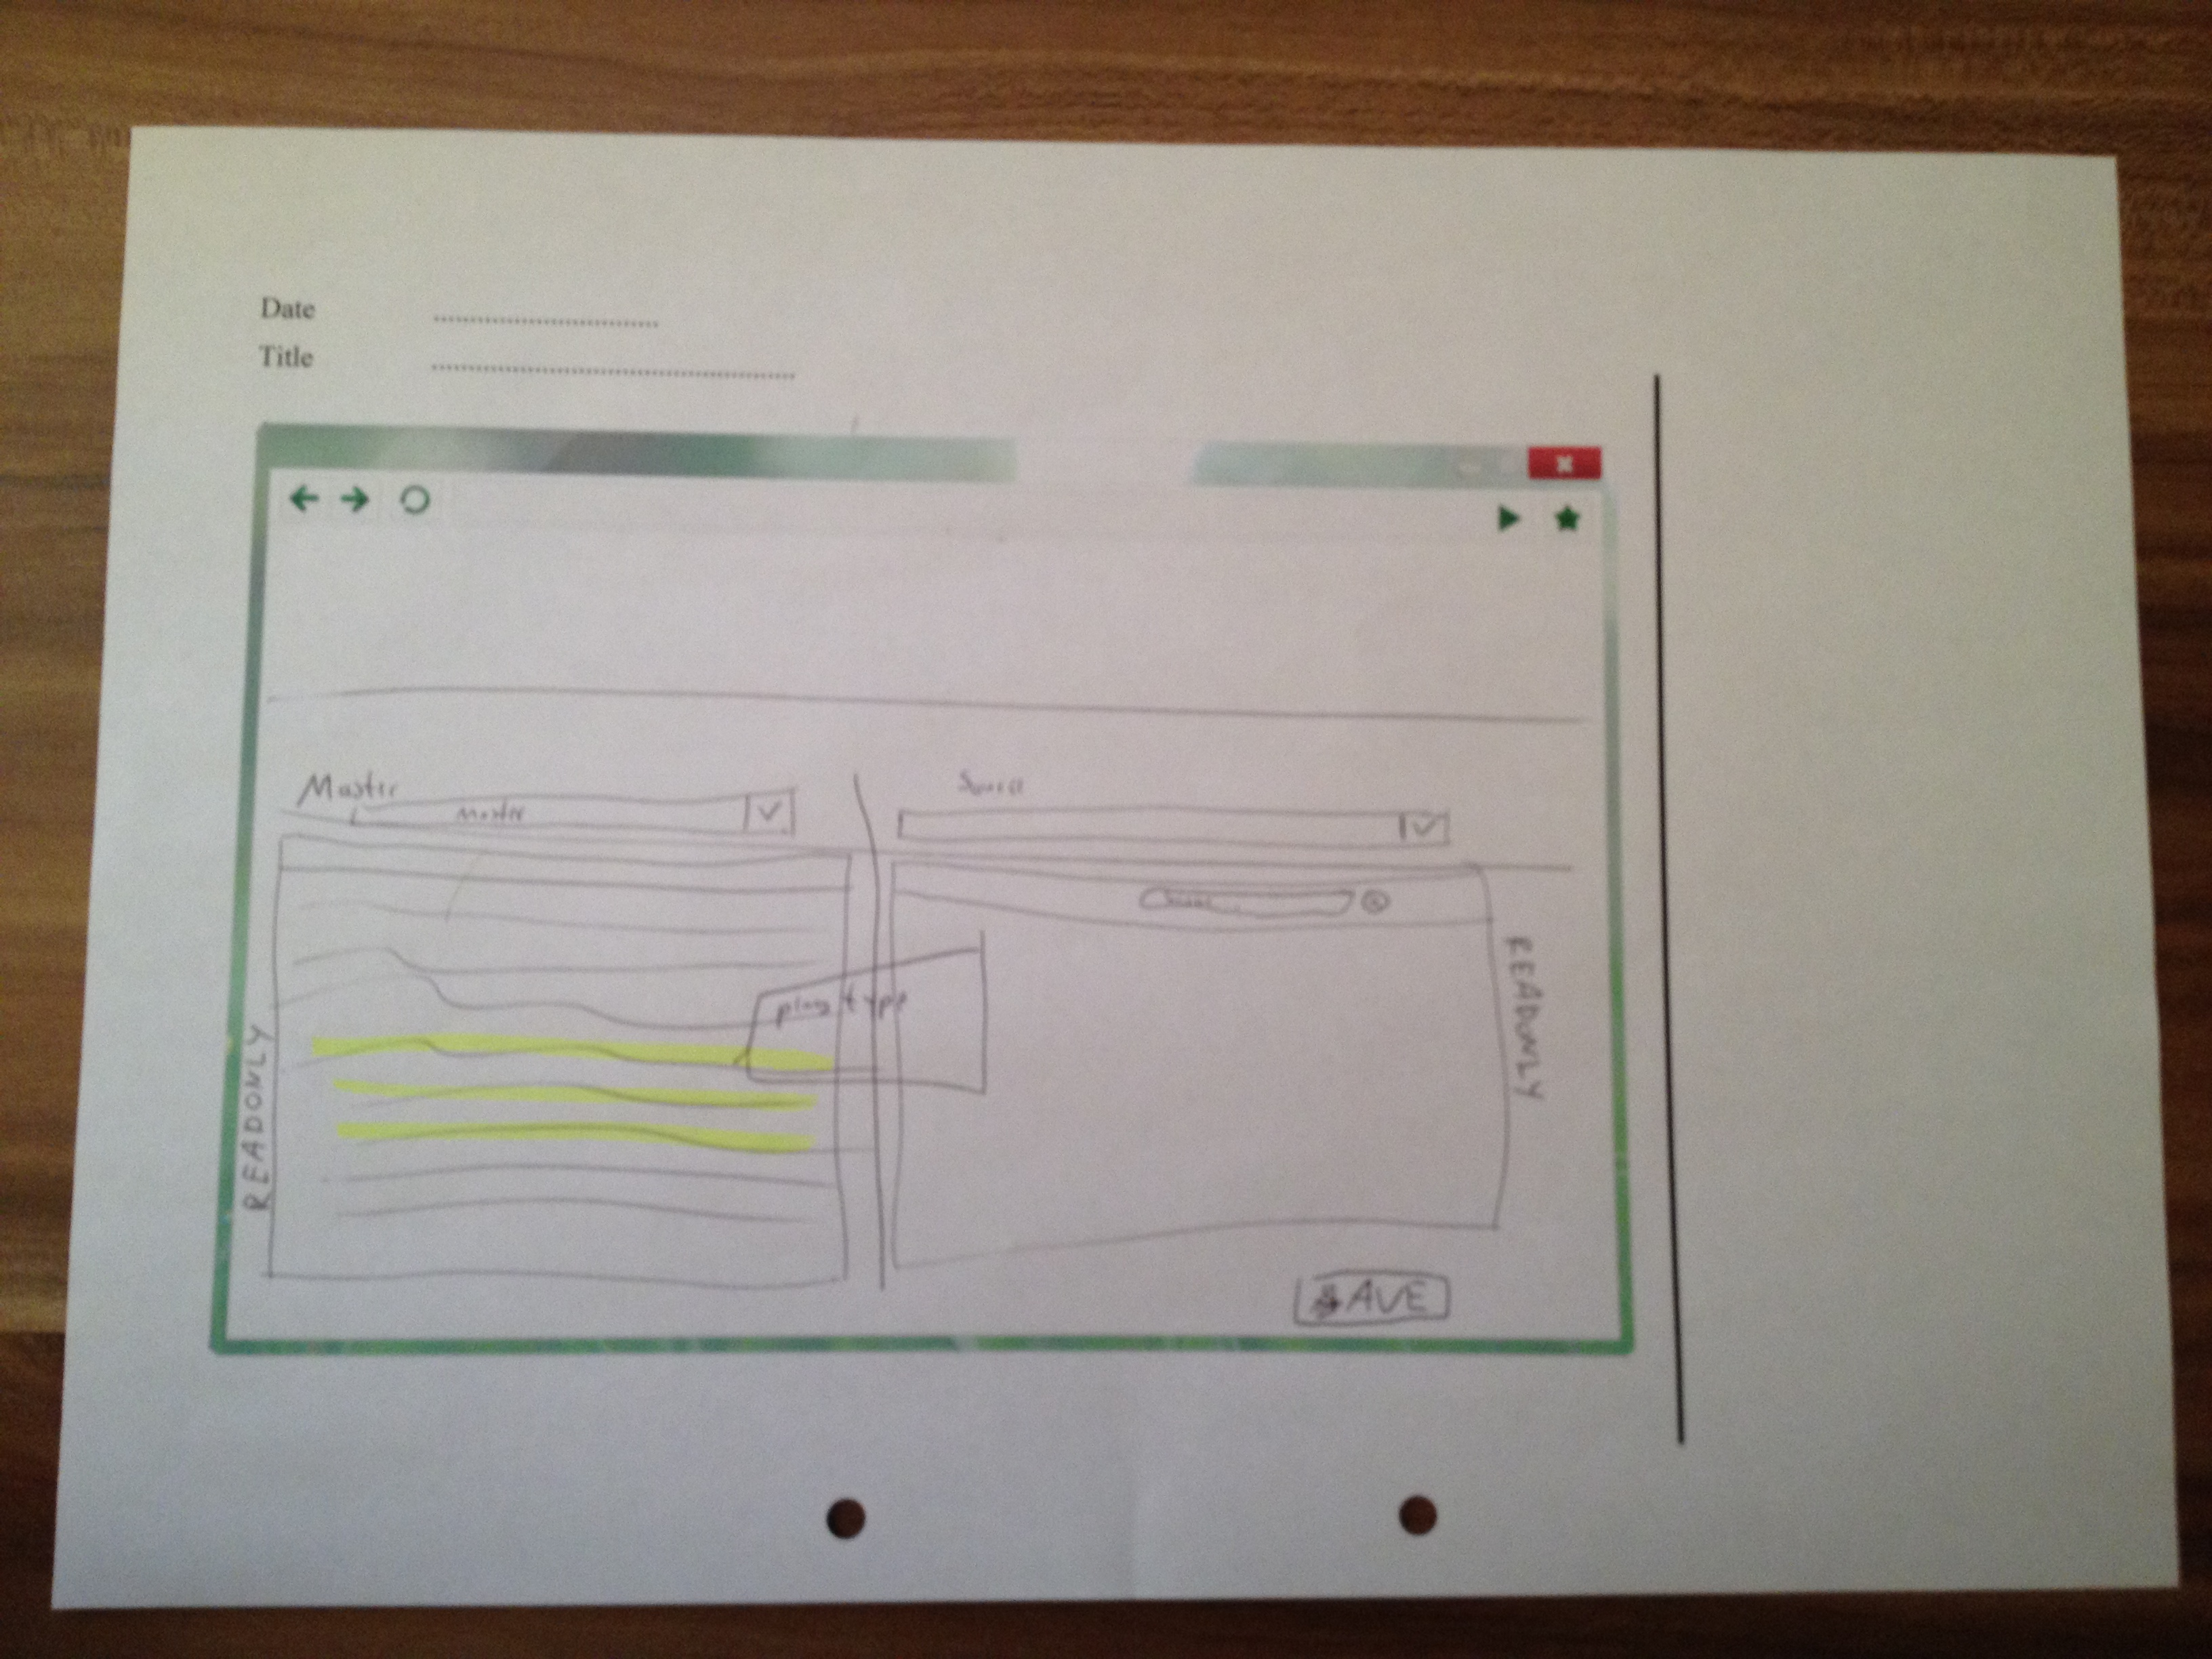
\includegraphics[width=\textwidth]{mockups/m_new_fragment.jpg}
  \caption{Mockup – New fragment – digitalized }
  \label{fig:1newCaseMockup}
\end{figure}

\begin{figure}[!h]
  \centering
    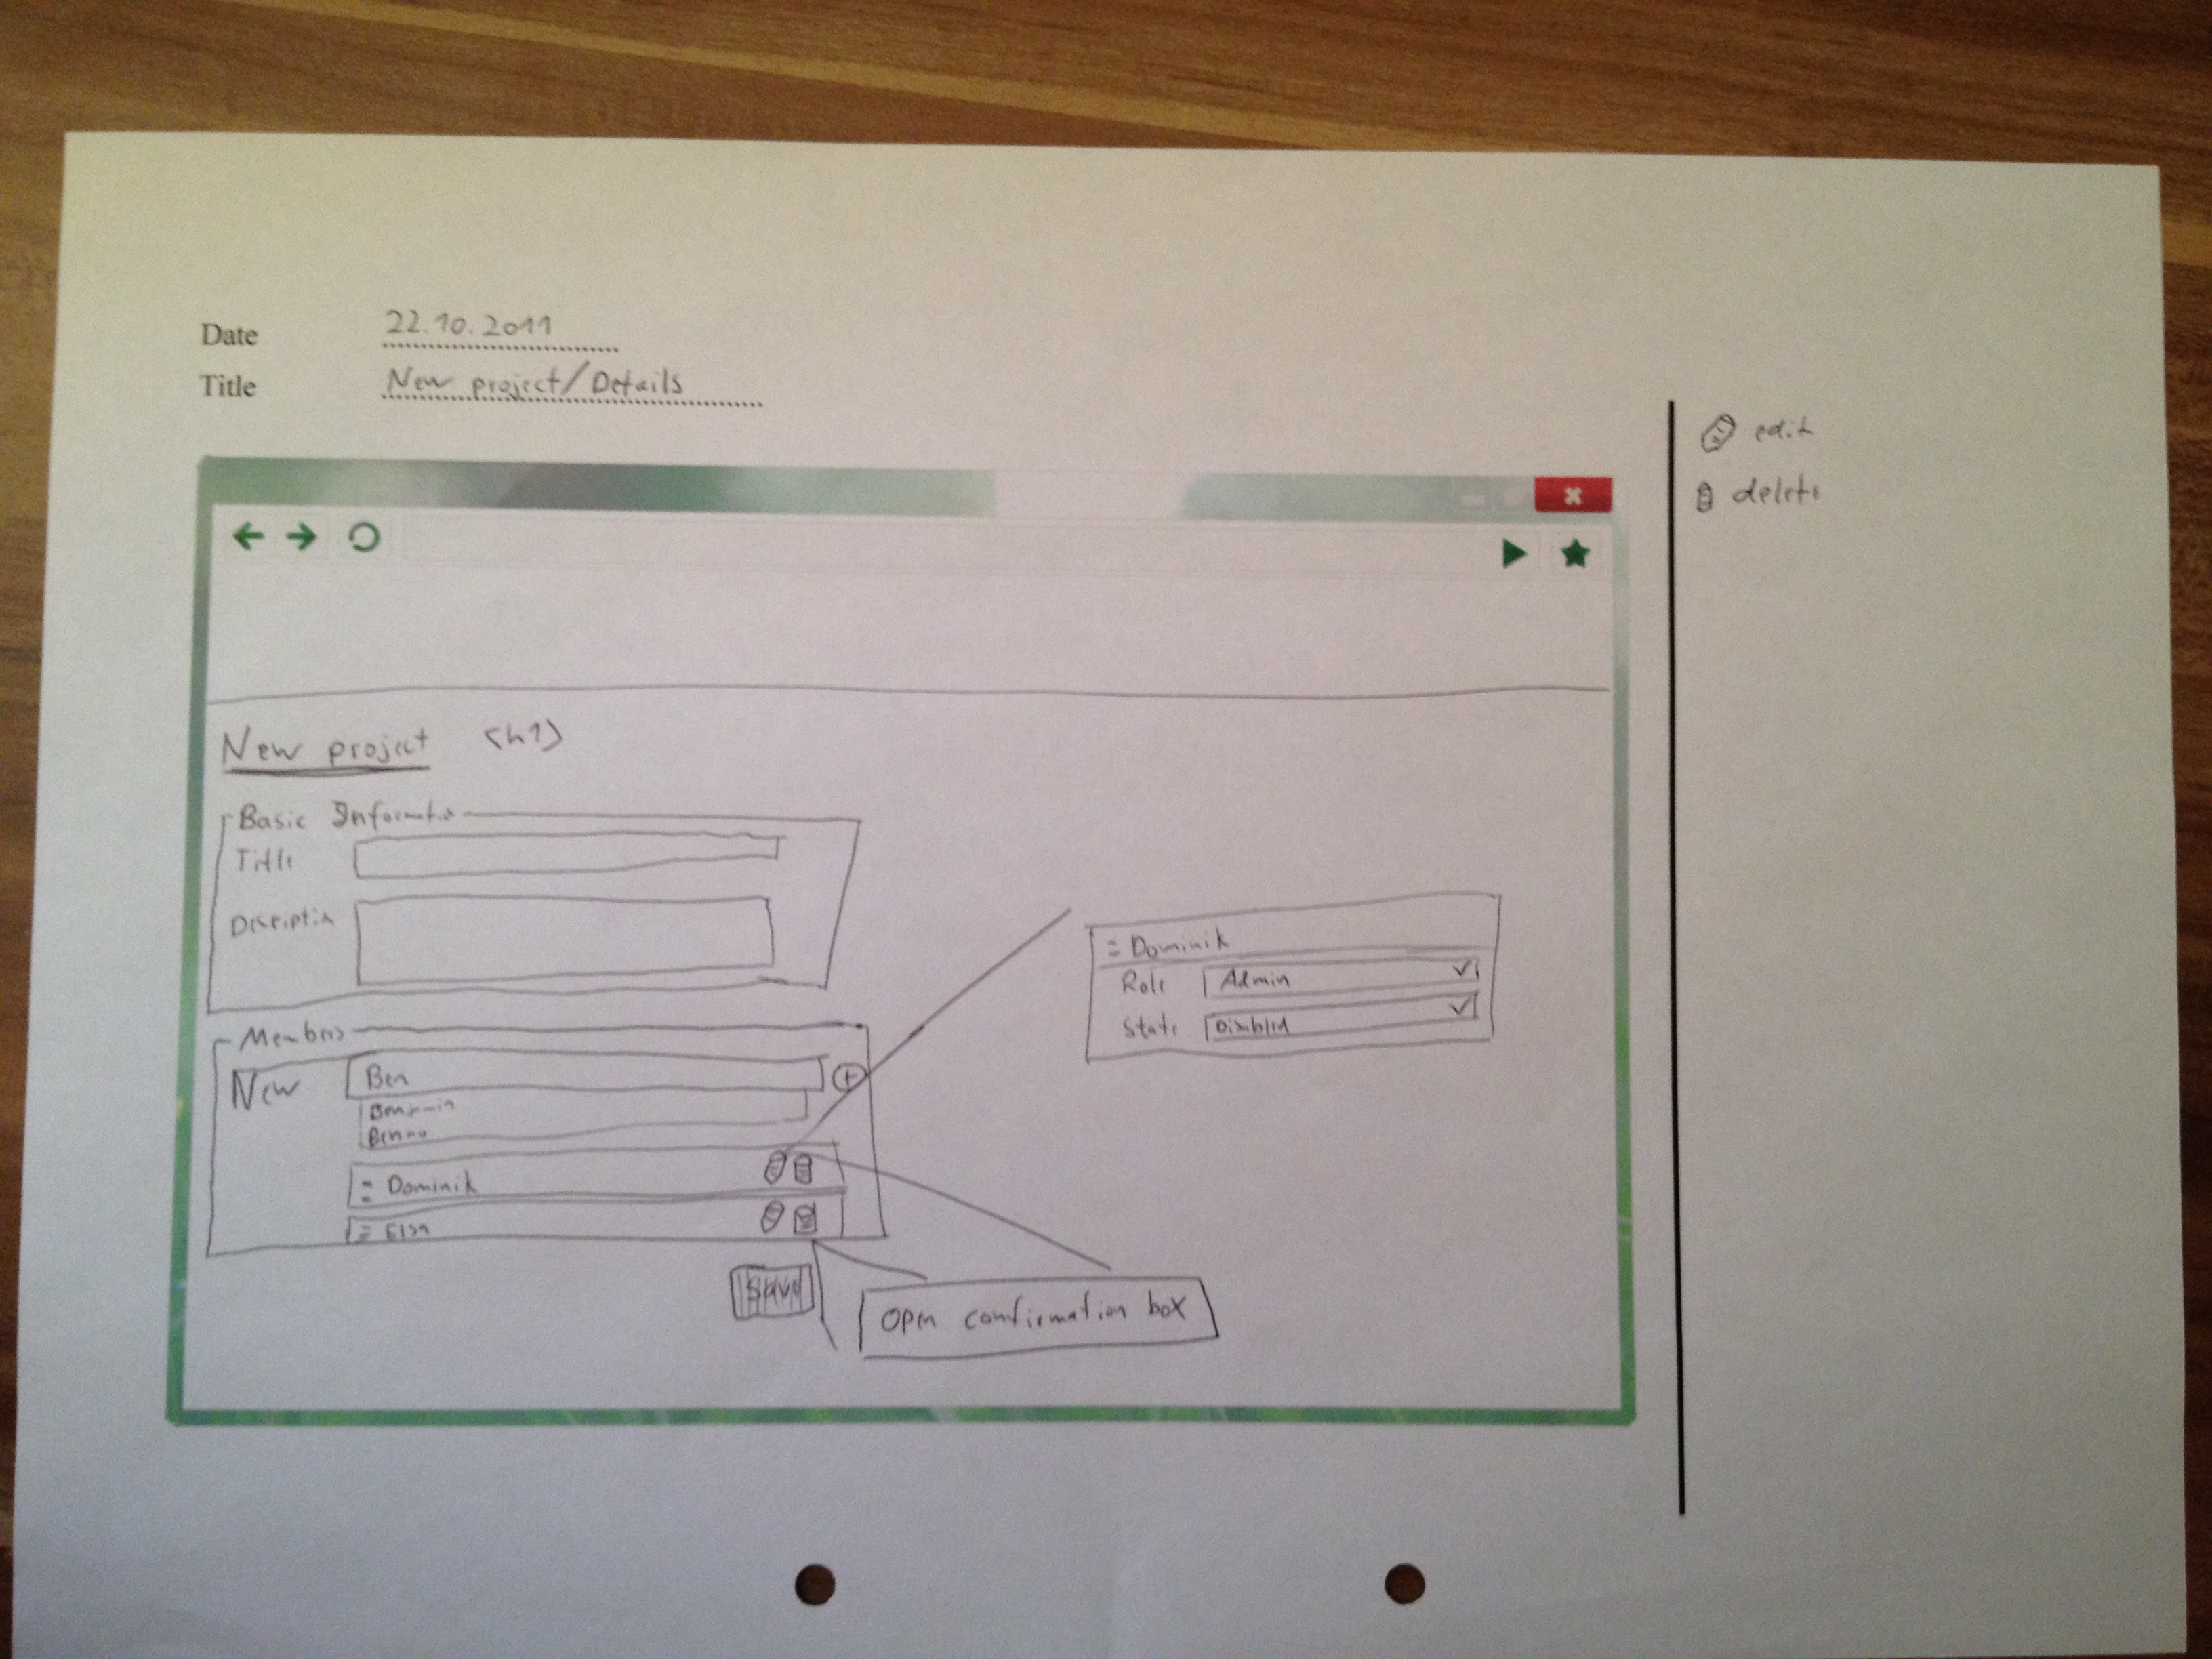
\includegraphics[width=\textwidth]{mockups/m_new_project.jpg}
  \caption{Mockup – New project – digitalized }
  \label{fig:mNewProjectMockup}
\end{figure}

\clearpage
\section{Digitalized}

\begin{figure}[htbp]
  \centering
    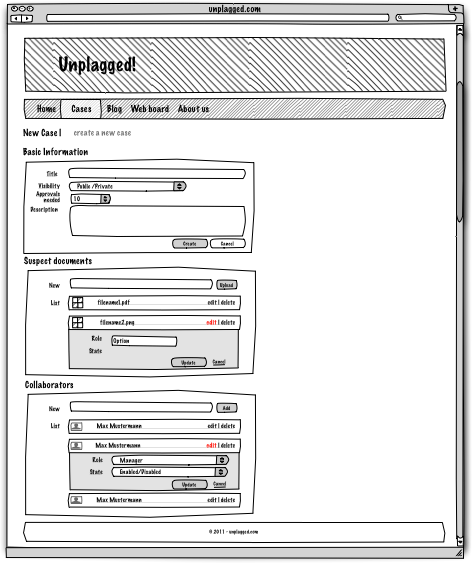
\includegraphics[width=0.86\textwidth]{mockups/1_new_case.png}
  \caption{Mockup – New case – digitalized }
  \label{fig:1newCaseMockup}
\end{figure}

\begin{figure}[!h]
  \centering
    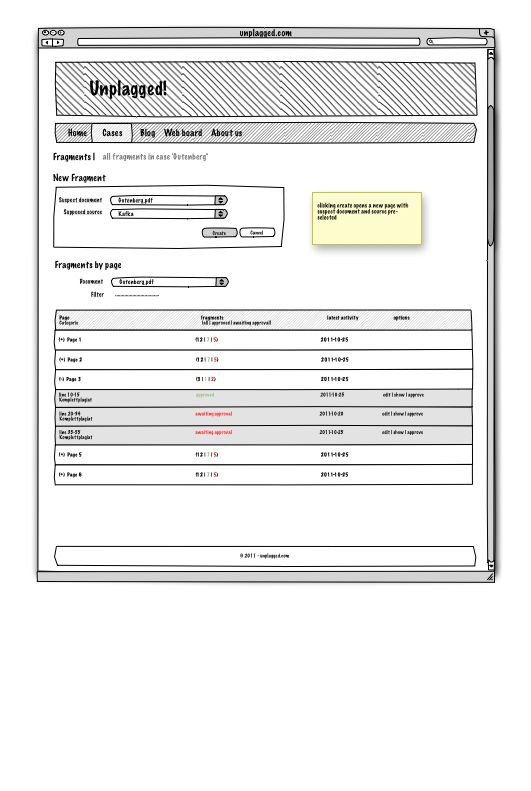
\includegraphics[width=\textwidth]{mockups/2_list_fragments.png}
  \caption{Mockup – List fragments – digitalized }
  \label{fig:2listFragmentsMockup}
\end{figure}

\begin{figure}[!h]
  \centering
    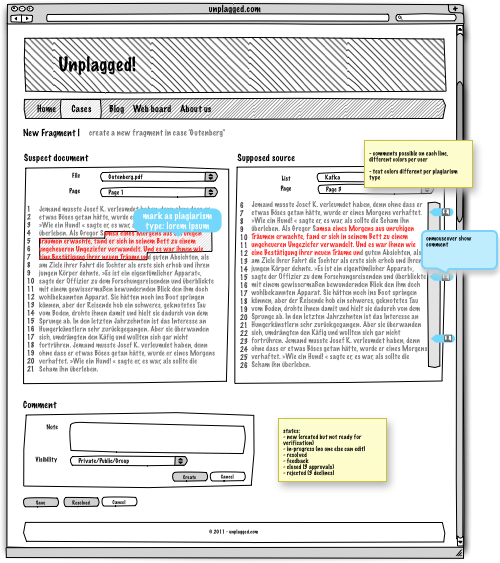
\includegraphics[width=\textwidth]{mockups/3_new_fragment.png}
  \caption{Mockup – New fragment – digitalized }
  \label{fig:3newFragmentMockup}
\end{figure}

\begin{figure}[!h]
  \centering
    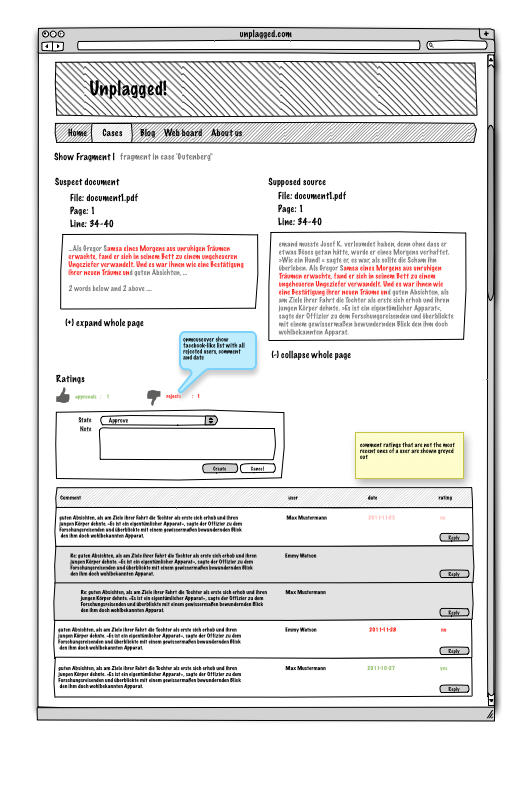
\includegraphics[width=0.97\textwidth]{mockups/4_show_fragment_for_approval.png}
  \caption{Mockup – Show fragment for approval – digitalized }
  \label{fig:4showFragmentForApprovalMockup}
\end{figure}

\begin{figure}[!h]
  \centering
    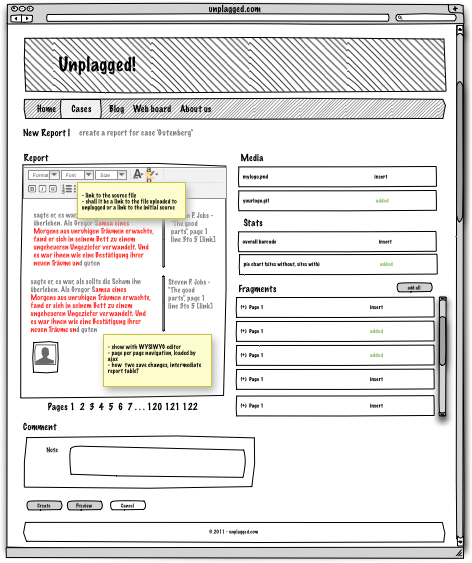
\includegraphics[width=\textwidth]{mockups/5_new_report.png}
  \caption{Mockup – New report – digitalized }
  \label{fig:5newReportMockup}
\end{figure}



\end{appendix}


\bibliography{biblio}

\end{document}